%%%%%% CMB-S4 Inflation Chapter  %%%%%%%%%%%%%%%%
 
\chapter{Inflation Physics from the Cosmic Microwave Background}
%\renewcommand*\thesection{\arabic{section}}

%%%%%%%%%%%%%%%%%%%%%%%%%%%%%%%%%%%%%%%%%%%%%%%%%%%%%%%%%%%
%%%%%%%%%%%%%%%%%%%%%%%%%%%%%%%%%%%%%%%%%%%%%%%%%%%%%%%%%%%
%%%%%%%%%%%%%%%%%%%%%%%%%%%%%%%%%%%%%%%%%%%%%%%%%%%%%%%%%%%
%%%%%%%%%%%%%%%%%%%%%%%%%%%%%%%%%%%%%%%%%%%%%%%%%%%%%%%%%%%


\begin{center}
{\small {\it (send feedback on this chapter to \href{mailto:s4\_inflation@cosmo.uchicago.edu}{s4\_inflation@cosmo.uchicago.edu})}}
\end{center}



\section{Introduction}
%The study of the polarization of the cosmic microwave background will bring additional information about both the gravitational and matter sectors of the primordial universe. However, for primordial gravitational waves there are clear theoretical thresholds that can be reached with this next generation instrument. We will use the tensor-to-scalar ratio as the primary inflationary science driver for the design.

With departures from complete homogeneity and isotropy at the $10^{-5}$ level and smaller, given a model, the statistical properties of temperature and polarization anisotropies of the CMB can be calculated to extremely high accuracy using perturbation theory. Their observation thus provides us with an opportunity for comparison with theory with a minimal amount of theoretical (calculational) uncertainty. The CMB provides us with a laboratory for the precision study of the origin of these small perturbations, which in turn is the study of the origins of all structure in the universe.

To date we have observed the result of {\em scalar} perturbations to the spacetime metric tensor. From these observations we have learned that the primordial scalar perturbations were nearly (but not quite) scale-invariant in the variance of their amplitudes, were consistent with Gaussianity, and, were made up of Fourier modes that all began their subhorizon dynamical evolution with the same temporal phase. 

These conclusions are also the predictions of the simplest models of cosmological inflation, and therefore the observations to date are a major success of the inflationary paradigm. 

But many questions remain. Did inflation actually occur? Are ground-state fluctuations truly the source of density perturbations? If inflation did occur, how did it occur? Was there a single effective field dominating the dynamics of both the background expansion and the perturbations, or were multiple fields involved? What is the connection of inflation physics to the rest of physics?

With CMB-S4 we have an opportunity to open up an entirely new window on the mechanism of the creation of these primordial perturbations: the {\em tensor} sector. We wish to stress the value of this new window in a model-independent manner, while simultaneously using the context of 
inflation to provide a more concrete framework for understanding the implications of the measurement of tensor perturbations. In the context of inflation, this new window offers a more direct probe of the dynamics of the inflationary expansion because the tensor perturbations are an inevitable consequence of the degrees of freedom of the spacetime metric obeying the uncertainty principle. The amplitude of the tensor perturbations depends only on the rate of expansion during inflation. In contrast, the amplitude of the scalar perturbations depends on both the amplitude and slope of the effective potential of the field responsible for inflation, and more generally on the sound speed of the inflaton field as well.

In addition to probing the origin of all structure in the universe, opening the tensor sector also opens up a probe of physics at length scales $\sim 10^9$ times smaller than those probed at the LHC. This small length scale is the size of the future horizon during inflation if it takes place at sufficiently high energies for us to observe the resulting tensor fluctuations. It is accessible because the immense amount of expansion during and since the inflationary epoch magnifies
these small length scales to ones of astrophysical size. If the tensor perturbations are detectable, we are already probing physics at these length scales via the scalar perturbations, but we cannot know this until the tensor perturbations are actually detected.

To date we only have upper limits on the amplitude of tensor perturbations, upper limits that are as strong as they can be from measuring temperature anisotropies. To detect the tensor perturbations we need to improve measurements of CMB polarization. On degree scales a polarization pattern known as B-mode polarization would reveal the existence of primordial tensor modes or gravitational waves. In the tensor sector, CMB-S4 will improve current constraints by almost two orders of magnitude. This is especially interesting because it allows this next generation instrument to reach theoretically well-motivated thresholds for the tensor-to-scalar ratio (the ratio of power in tensor modes to power in scalar modes), which consequently serves as the primary inflationary science driver for the design. 

Inflation predicts B-mode fluctuations  sourced by primordial gravitational waves. But more generally, the B-mode signal again carries information about both the spectrum of primordial perturbations in the tensor (and vector) components of the metric and any physics that affected the evolution of those modes once they re-entered the horizon.  

{\it A detection of primordial gravitational waves would open a completely new window on the physical processes of the early universe and reveal a new scale of particle physics far above those accessible with terrestrial particle colliders. }

If the overall amplitude of the B-mode signal is large enough to be detected at high significance by the CMB S4 instrument, we will be able to begin further characterizing the statistics of the perturbations. Investigating the scale-dependence of the amplitude of fluctuations and their Gaussianity will allow us to determine if the signal is consistent with the amplification of quantum vacuum fluctuations of the metric during inflation. If CMB S-4 measurements are consistent with a nearly scale invariant and a weakly non-Gaussian spectrum, a detection would
\begin{itemize}
 \item Identify the energy scale of inflation. 
  \item Provide strong evidence that gravity is quantized, at least at the linear level.
 \item Provide strong evidence that the complete theory of quantum gravity must accommodate a Planckian field range for the inflaton.
\end{itemize}

Departures from a nearly scale-invariant, Gaussian spectrum would reveal new physics beyond the simplest inflationary models. Existing models propose some examples of predictions from a richer inflationary or post-inflationary sector, which would be tested. However, given the lack of observational constraints on physics at such high energy scales there is also enormous discovery potential. Polarization data also provides consistency checks on the current dominant theoretical framework, including model-independent constraints on the graviton mass and constraints on alternatives to inflation.

In the absence of a detection, CMB-S4 would put some of the most significant constraints on inflation models to date, ruling out large classes models. {\bf What else should be stated here?}

{\bf Insert paragraph emphasizing inflation-related gains from the scalar sector with CMB-S4.}

In Section~\ref{sec:basics} we provide a basic introduction of the inflationary paradigm in its simplest form. In Section \ref{sec:detection} we review in detail what a detection of primordial gravitational waves would mean and what follow-up measurements should or could be done to further characterize any signal. Section \ref{sec:upperLimits} explains the implications of a robust upper limit of $r<0.001$. Section \ref{sec:needs} lays out what is required to achieve that goal. The final two sections describe the significant gains CMB-S4 will allow in constraining other aspects of the primordial universe, both standard and more speculative. These include characterizing the scalar power spectrum, constraining curvature, non-Gaussianity, isocurvature modes, further probes of CMB `anomalies' and tests/constraints of cosmic strings.
 

%Recent reviews \cite{Kamionkowski:2015yta}.

\section{Basics of Cosmological Inflation}
\label{sec:basics}

Inflation is, by definition, a period of accelerating expansion. As explained in Fig.~\ref{fig:PTfigs}, an accelerating universe has a causal structure very different from that of a decelerating universe. In a decelerating universe, a pair of separated comoving particles evolves from being causally disconnected -- in which case the particles, unable to influence each other, are said to be superhorizon -- to being causally connected, or subhorizon. In an accelerating universe, the opposite occurs. In the inflationary scenario, the universe undergoes an accelerating stage, which is followed by a long period of deceleration.


\begin{figure}[ht]
\centering
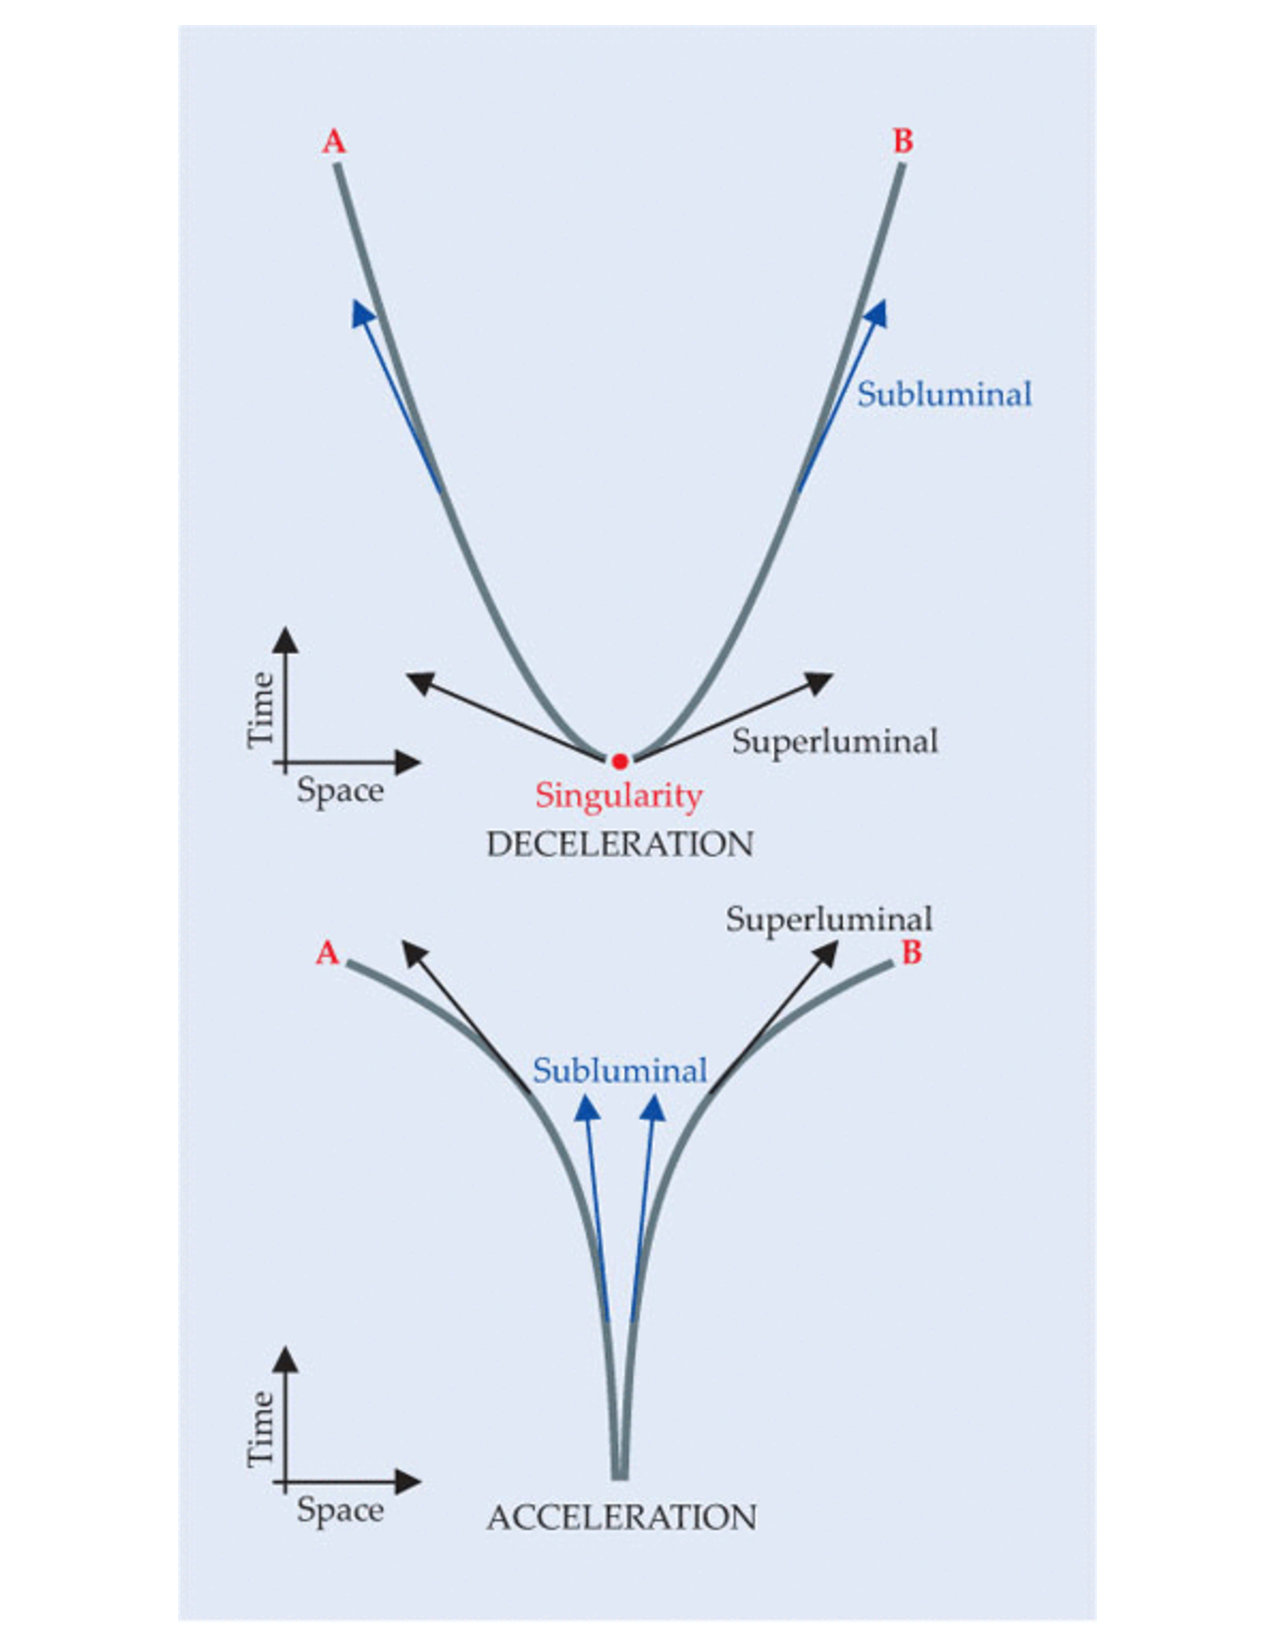
\includegraphics[width=0.36\textwidth]{Inflation/CausalStructure.pdf}
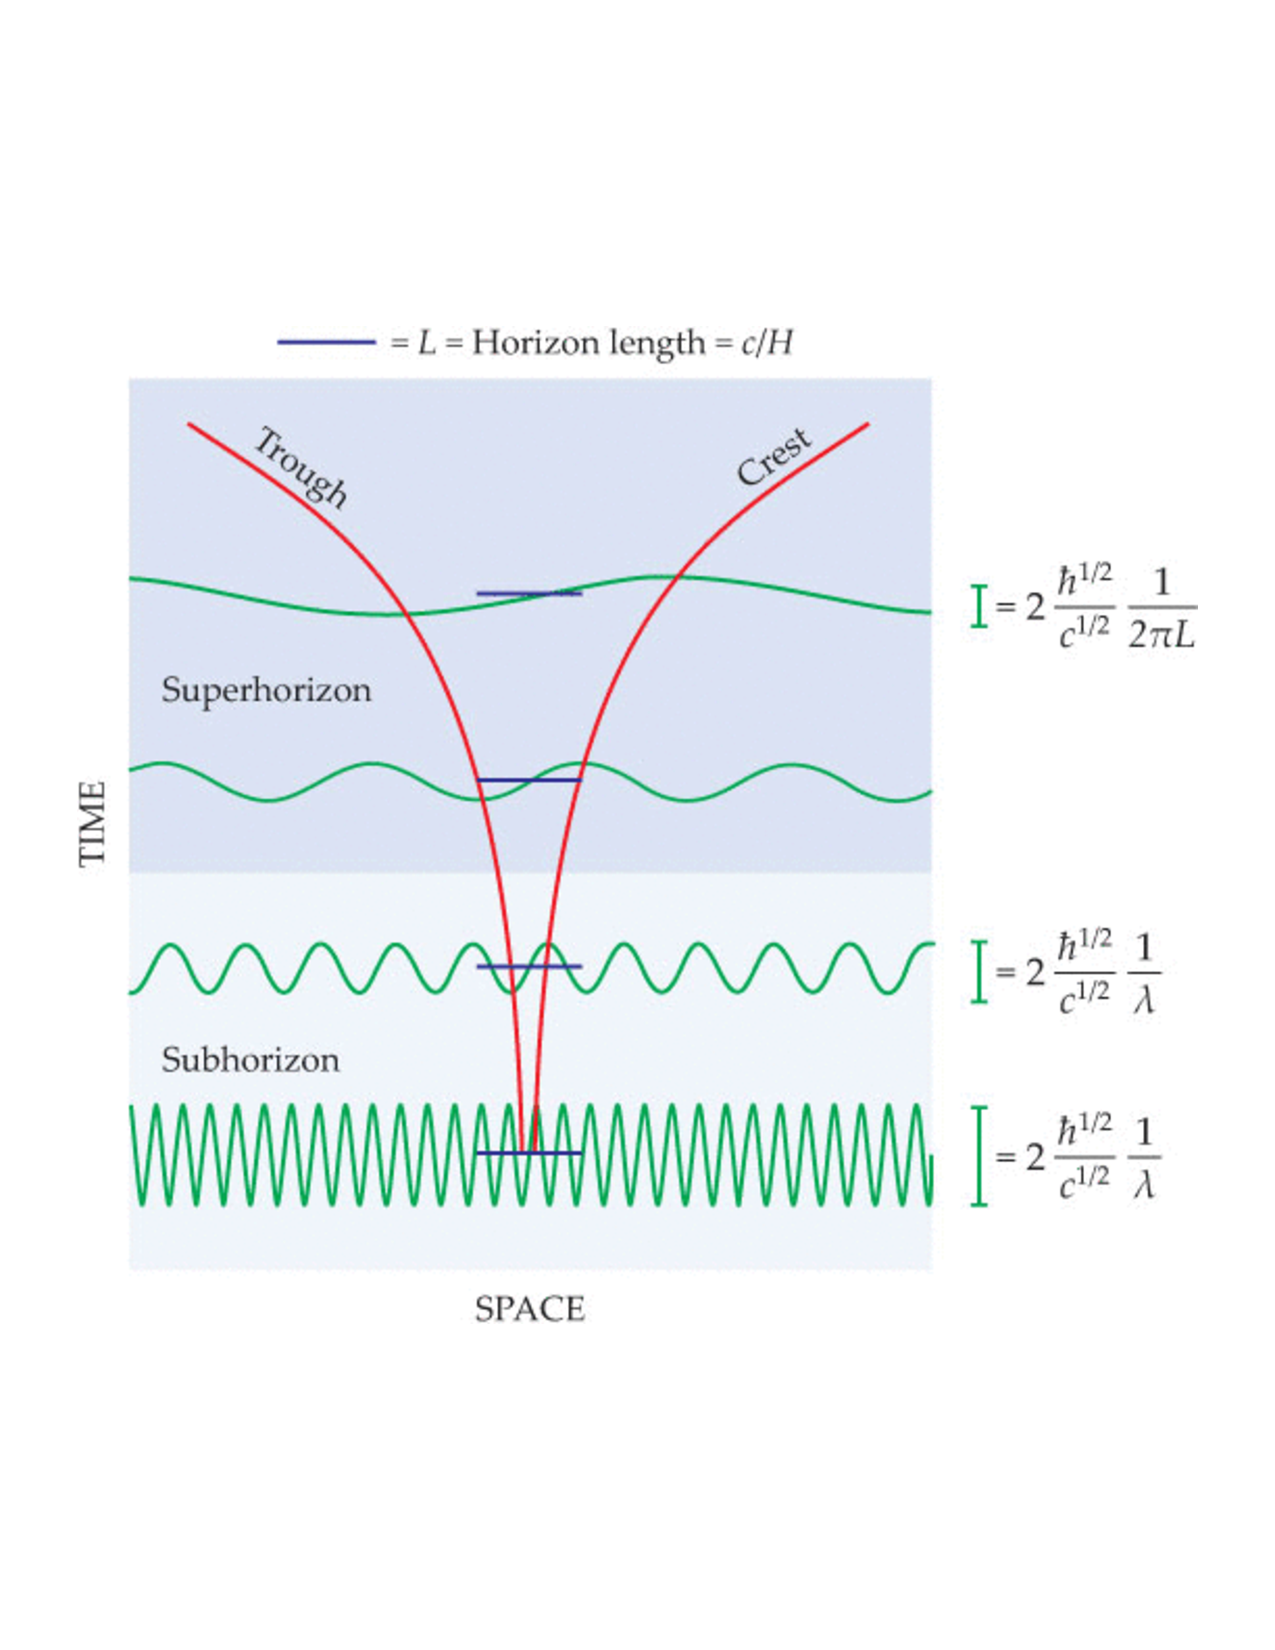
\includegraphics[width=0.36\textwidth]{Inflation/QuantumFluctuations.pdf}
\caption{{\bf Left panel}: In an expanding universe, the distance between two separated points increases over time, simply due to the expansion of the space between them. The two panels here show the spacetime trajectories of two comoving points, A and B. For the decelerating expansion illustrated in the top panel, the separation rate is greater in the past and even exceeds the speed of light at sufficiently early time. Thus A and B go from being out of causal contact—unable to influence each other—to being in causal contact. In an accelerating universe, the separation rate is smaller in the past; the two points go from being in causal contact to being out of causal contact. In the inflationary universe scenario, an early epoch of acceleration—the inflationary era—smoothly maps onto a long period of deceleration. Thus two points can go from being in causal contact to out of causal contact and, much later, back into causal contact. {\bf Right panel}:
Fluctuations in the value of the inflaton field, which is responsible for the accelerating expansion of the cosmos, evolve differently, depending on whether their wavelength $\lambda$ is less than or greater than the horizon length $L = c/H$. When $\lambda \ll L$, the uncertainty principle limits how smooth the field can be. As a result, the amplitude of the fluctuation is inversely proportional to $\lambda$ and thus decreases as the universe expands. (The influence of the uncertainty principle is reflected by the appearance of Planck’s constant $\hbar$ in the expression for the amplitude.) As $\lambda$ becomes larger than the horizon, the crest and trough of the wave cease to be in causal contact, so the amplitude stops evolving. For superhorizon evolution, its asymptotic value corresponds to replacing the wavelength in the subhorizon case with $2\pi L$. Eventually, cosmic expansion stretches the fluctuations to astrophysically large length scales.
}
\label{fig:PTfigs}
\end{figure}


In view of the early period of accelerating expansion, two separated regions in the universe that are now causally disconnected could have been able to interact with each other during the inflationary epoch. Causally connected perturbations in those two regions -- for example, an underdensity in one and an overdensity in the other -- could thus have been created at very early times. Quantum mechanics provides a mechanism for generating such perturbations, and in fact makes them unavoidable. Quantum mechanical fluctuations initially created with subnuclear wavelengths are stretched by the cosmic expansion to millimeter length scales within a tiny fraction of a second; at present they are astrophysically large. Thus observations of cosmic structure give us an opportunity to probe physics on extremely small length scales.

Accelerating expansion requires the universe to have an energy density that dilutes relatively slowly with expansion. In inflationary models, such an energy density is usually obtained via the introduction of a new field $\phi$, called the inflaton field with Lagrangian density, in the simplest cases, given by
\begin{equation}
{\cal L} = \frac{1}{2} \partial_\mu \phi \partial^\mu \phi - V(\phi)
\end{equation}
where $V(\phi)$ is a potential energy density. 

A generic inflaton field configuration will not lead to inflation. But if there is a large enough patch of space in which $\phi$ takes values for which the potential is sufficiently flat, $\phi$ will rapidly evolve to satisfy the ``slow-roll condition'', $\frac{1}{2} \left(d\phi/dt\right)^2 \ll V(\phi)$. When both the spatial and temporal derivatives of the inflaton field are small, $V(\phi)$ is nearly constant in time and makes the dominant contribution to the energy density. Under such conditions, and given the Friedmann equation $\dot a/a \propto \sqrt{\rho}$, the patch inflates. In the limit that the energy density is completely constant in time, the scale factor grows as $e^{H t}$, and points separated by more than $c/H$ are causally disconnected.

A standard assumption in the calculation of inflationary perturbation spectra is that the field is as smooth as it possibly can be, and still be consistent with the uncertainty principle. As Fig.~\ref{fig:PTfigs} shows, these fluctuations will be stretched to astrophysically large length scales by cosmic expansion. In an inflationary scenario quantum fluctuations provide the initial seeds of all structure in the universe. 

As $\phi$ rolls toward the potential minimum, $V(\phi)$ eventually becomes smaller than $\frac{1}{2}(d\phi/dt)^2$; the slow-roll condition is no longer met, and inflation ends. Decays of the inflaton to other particles -- irrelevant during inflation because the decay products were quickly diluted by expansion -- then become important. The remaining energy in the $\phi$ field converts to a thermal bath of the particles of the standard model, and perhaps other particles as well.

The small but nonzero spatial fluctuations in $\phi$ cause inflation to end at different times in different locations. In those regions where inflation ends relatively early, the mass density is lower due to the extra expansion that the region has undergone since the end of inflation. Thus the slightly different expansion histories of different locations result in density differences; those small density perturbations eventually grow under the influence of gravity to create all the structures we observe in the universe today.

The spacetime metric itself, at least in a linearized treatment, presumably obeys the uncertainty principle as well. As a result, we expect a nearly scale-invariant spectrum of gravitational waves to be produced during inflation as well. Just as with fluctuations of the inflaton field, they obey an uncertainty principle and, in the course of superluminal expansion, have their amplitude set to a value proportional to the Hubble parameter $H$ during inflation. Detecting the influence of that gravitational-wave background on the CMB would allow cosmologists to infer $H$ and hence the energy scale of the inflationary potential; observations of density perturbations, by contrast, provide a relatively indirect look at the inflationary era. As emphasized in the previous section, CMB-S4 is poised to detect, or place interesting upper limits, on the amplitude and spectrum of inflation-produced gravitational waves via their signature in B-mode polarization. 


\section{Implications of a detection of primordial gravitational waves with CMB-S4}
\label{sec:detection}
The overall evolution of the universe is well modeled by a Friedmann-Lema\^{\i}tre-Robertson-Walker line element
\begin{equation}
ds^2=-dt^2+a^2(t)\left[\frac{dr^2}{1-kr^2}+r^2d\Omega^2\right]\,,
\end{equation}
where $k=\pm1$ allows for spatial curvature and the time evolution is specified by the scale factor, $a(t)$. The Hubble parameter, $H=\dot{a}/a$, gives the rate of expansion of the universe. 
%Current data is consistent with a spatially flat universe, and we will assume spatial flatness ($k=0$) for most of the discussion. However, we will return to constraints on the curvature in Section xxx.  

The existence of primordial Helium and the cosmic microwave background radiation provide strong evidence for a hot big bang, a period during which the universe was dominated by radiation before it became dominated by matter and eventually dark energy. In the context of general relativity, observations of the cosmic microwave background furthermore provide strong evidence for a period preceding the hot big bang during which the co-moving Hubble radius, $(a|H|)^{-1}$, was decreasing with time: the measured average CMB temperature and the statistics of the measured anisotropies are the same over regions that otherwise share no causal history. 

%Arguably the most significant discrepancy between the predictions of a generic hot big bang model and our observed sky is the horizon problem: the measured average CMB temperature and the statistics of the measured anisotropies are the same over regions that share no causal history. Models for the primordial universe attempt to give a causal (and ideally also a `natural') explanation for the observed homogeneity on scales greater than a few degrees by postulating an early era where the co-moving Hubble radius, $(a|H|)^{-1}$ is decreasing with time. In an expanding universe this requires an era of accelerated expansion, $\ddot{a}>0$. The matter field that sources this expansion should have equation of state $w\approx -1$, which is minimally provided by a single scalar field whose energy density is predominately determined by its potential.

In an expanding universe a decreasing co-moving Hubble radius requires an era of accelerated expansion, $\ddot{a}>0$, cosmic inflation. Such a period will drive the spatial curvature close to zero, in good agreement with current observations. Thus, we will assume spatial flatness and set $k=0$ for most of the discussion, but will return to constraints on the curvature in Section \ref{sec:other_topics}. Since the period of cosmic inflation must end, there must exist a clock, or scalar degree of freedom. According to the uncertainty principle this clock must fluctuate, generating density perturbations that are adiabatic. In the most economic scenarios, these density perturbations are the seeds that grow into the anisotropies observed in the cosmic microwave background radiation and the stars and galaxies around us. Other degrees of freedom could, of course, also be present during this phase and might even be responsible for the generation of density perturbations we observe. 

%{\bf (Mention isocurvature modes here?)}

Alternatively, the phase of decreasing co-moving Hubble radius could have occurred during a period of decelerating contraction which must then be followed by a bounce as in the ekpyrotic or matter bounce scenarios \cite{Khoury:2001wf,Khoury:2001bz,Steinhardt:2001st,Nayeri:2005ck,Brandenberger:2012zb,Cai:2014jla,deHaro:2015wda}. 
% The matter field that sources this expansion should have an equation of state $w\approx -1$, which is minimally provided by a single scalar field whose energy density is predominately determined by its potential.

%The remarkable feature of inflation is that once an evolving scalar field is invoked to source the background accelerated expansion, quantum fluctuations during inflation inevitably generate post-inflationary metric perturbations. 
For these early times, the ADM formalism provides a convenient parametrization of the line element
\begin{eqnarray}
\label{eq:metric}
ds^2&=&-N^2dt^2 +h_{ij}(dx^i+N^idt)(dx^j+N^jdt)\,\nonumber\\
h_{ij}&=&a^2(t)[e^{2\zeta}\delta_{ij}+\gamma_{ij}]\,.
\end{eqnarray}

The equations of motion for $N$ (the lapse) and $N^i$ (the shift) are the Hamiltonian and momentum constraints, while $\zeta$ ($=-\mathcal{R}$ in the {\it Planck} collaboration papers) and $\gamma_{ij}$ contain the dynamical scalar and tensor degrees of freedom. In scenarios with matter sources other than a scalar field there may also be vector perturbations. These rapidly decay and can be neglected unless they are actively sourced in the post-inflationary universe, e.g. by cosmic strings.

%RF perhaps add Fourier transform and define horizon exit, freeze out at this point
Because the equations of motion are invariant under translations and the perturbations are linear or nearly so, it is convenient to work with the Fourier transforms
\begin{equation}
\zeta(t,\vec{x})=\int \frac{d^3 k}{(2\pi)^3}\zeta(t,\vec{k})e^{i \vec{k}\cdot\vec{x}}+h.c.\qquad{\rm and}\qquad\gamma_{ij}(t,\vec{x})=\sum\limits_s\int\frac{d^3k}{(2\pi)^3}\gamma_s(t,\vec{k})e_{ij}(\vec{k},s)e^{i \vec{k}\cdot\vec{x}}+h.c.\,,
\end{equation}
where $e_{ij}(\vec{k},s)$ is the transverse traceless polarization tensor for the graviton. The solutions oscillate when the modes are deep inside the horizon, $k\gg aH$. By definition, the modes exit the horizon when $k=aH$ and in single-field models approach a constant outside the horizon when $k\ll aH$.

The statistical properties of the scalar and tensor fluctuations, $\zeta$ and $\gamma_s$, at times sufficiently late so that they have frozen out provide the link between the primordial era and the observed CMB today as well as other probes of the structure of the late universe. For a universe that is statistically homogeneous and isotropic and in which the primordial fluctuations are Gaussian, the information about the statistical properties is contained in the two-point correlation functions

\begin{eqnarray}
\langle\zeta(\vec{k})\zeta(\vec{k}^{\prime})\rangle&=&(2\pi)^3\delta^3(\vec{k}+\vec{k}^{\prime})\frac{2\pi^2}{k^3}\mathcal{P}_{\zeta}(k)\nonumber\\
\langle\gamma_s(\vec{k})\gamma_{s^{\prime}}(\vec{k}^{\prime})\rangle&=&(2\pi)^3\delta_{ss^{\prime}}\delta^3(\vec{k}+\vec{k}^{\prime})\frac{2\pi^2}{k^3}\frac{1}{2}\mathcal{P}_{t}(k)\nonumber\\
\end{eqnarray}
where the factor of $1/2$ in the second to last line accounts for the fact that the measured power includes contributions from each of the two graviton polarizations. In single field slow-roll inflation, the gauge invariant combination of metric and scalar field fluctuations that is conserved outside the horizon has the power spectrum
\begin{equation}
\label{eq:inf_Pzeta}
\mathcal{P}_{\zeta}(k)=\frac{1}{2\epsilon M_p^2}\left.\left(\frac{H}{2\pi}\right)^2\right|_{k=aH}
\end{equation}
where $\epsilon=-\dot{H}/H^2$ is the first slow-roll parameter, and $M_p=1/\sqrt{8\pi G}$ is the reduced Planck mass. As indicated, the Hubble parameter and $\epsilon$ are to be evaluated at horizon exit when the wavenumber $k$ is equal to the inverse comoving Hubble radius. In the absence of additional sources, the tensor power spectrum generated by inflation is
\begin{equation}
\label{eq:inf_Pt}
\mathcal{P}_{t}(k)=\frac{8}{M_p^2}\left.\left(\frac{H}{2\pi}\right)^2\right|_{k=aH}
\end{equation}

It is convenient to introduce the logarithmic derivatives of these power spectra 
\begin{equation}\label{eq:specind}
n_s(k)-1\equiv\frac{d\ln \mathcal{P}_{\zeta}}{d\ln k}\qquad{\rm and}\qquad n_t(k)\equiv \frac{d\ln \mathcal{P}_t}{d\ln k}\,.
\end{equation}
If the Hubble rate and slow-roll parameter only weakly depend on time as in slow-roll inflation, these will be $n_s(k)\approx 1$ and $n_t(k)\approx 0$ and can be expanded around a pivot scale $k_\star$ accessible by the CMB
\begin{equation}
n_s(k)-1=n_s-1+\left.\frac{dn_s(k)}{d\ln k}\right|_{k_\star}\ln(k/k_\star)+\dots\qquad{\rm and}\qquad n_t(k)=n_t+\left.\frac{dn_t(k)}{d\ln k}\right|_{k_\star}\ln(k/k_\star)+\dots
\end{equation}
In this approximation, the power spectra are
\begin{eqnarray}\label{eq:power_spectra_power_law}
\mathcal{P}_{\zeta}(k)&=& A_s\left(\frac{k}{k_\star}\right)^{n_s-1+\frac{1}{2}\left.\frac{dn_s}{d\ln k}\right|_{k=k_\star}\ln(k/k_\star)+\dots}\,,\nonumber\\
\mathcal{P}_{t}(k)&=& A_t \left(\frac{k}{k_\star}\right)^{n_t+\frac{1}{2}\left.\frac{dn_t}{d\ln k}\right|_{k=k_\star}\ln(k/k_\star)+\dots}\,,
\end{eqnarray}
%\begin{equation}\label{eq:specind}
%\mathcal{P}_{\zeta}(k)\equiv A_s\left(\frac{k}{k_\star}\right)^{n_s-1}\qquad{\rm and}\qquad\mathcal{P}_{t}(k)\equiv A_t \left(\frac{k}{k_\star}\right)^{n_t}\,,
%\end{equation}
where $A_s$, $A_t$ are the scalar and tensor amplitudes, and $n_s$ and $n_t$, are the scalar and tensor spectral index, respectively, both at the pivot scale. 
The tensor-to-scalar ratio, $r$, is the relative power in the two types of fluctuations at a chosen pivot scale $k_\star$ accessible by the CMB
\begin{equation}
r=\frac{A_t}{A_s}\;.
\end{equation}

The power spectra of $\zeta$ and $\gamma_s$ are time-independent as long as the modes are outside the horizon, and only begin to evolve once the modes of interest re-enter the horizon at late times. In particular, they set the initial conditions for the system of equations governing the time evolution of the universe from around $10^9$ K when electrons and positrons have annihilated to the present. To exhibit the link between the primordial perturbations and late time observables explicitly, note that in a spatially flat universe, the contributions of primordial scalar perturbations to the angular power spectra of temperature or E-mode anisotropies are given by
\begin{equation}
C^{(S)}_{XX,\ell}=\int \frac{dk}{k}\mathcal{P}_\zeta(k)\left|\int\limits_0^{\tau_0} d\tau S_X^{(S)}(k,\tau)j_\ell(k(\tau_0-\tau))\right|^2\,,
\end{equation}
where $j_\ell$ is a spherical Bessel function that encodes the (spatially flat) geometry of the universe and $S_X^{(S)}(k,\tau)$ with $X=T,E$ are source functions that encode the evolution of the modes in the hot big bang universe (in particular, the physics of recombination is very important for B-modes).
% and $\mathcal{P}_\zeta(k)$ is the power spectrum of initial conditions of primordial scalar perturbations as a function of the (comoving) momentum of the modes. 
At linear order, scalar perturbations only contribute to angular power spectra of temperature and E-mode polarization and the cross-spectrum of temperature and E-mode polarization, while the tensor perturbations in addition generate B-mode polarization. The primordial contribution of the tensor perturbations to the angular power spectrum of B-modes is 
\begin{equation}
C_{BB,\ell}=\int \frac{dk}{k}\mathcal{P}_t(k)\left|\int\limits_0^{\tau_0} d\tau S_B^{(T)}(k,\tau)j_\ell(k(\tau_0-\tau))\right|^2\,.
\end{equation}
where $S_B^{(T)}(k,\tau)$ is the appropriate source function. 

At present, bounds on the tensor contribution to the temperature and E-mode anisotropies are comparable to constraints on the tensor-to-scalar ratio from B-mode observations. The former constraints are now cosmic variance limited. There is no limit on the latter from cosmic variance, and improvements and a potential detection with CMB-S4 will rely on measurements of B-mode polarization on degree scales.

Constraints on the amplitude of primordial tensor modes already strongly disfavor once popular inflationary models like minimally coupled chaotic inflation with a quadratic potential. In the next few subsections we will discuss in detail what a detection of primordial gravitational waves would imply for theories of the primordial universe. 

%but it is also important to note that a detection would rule out contracting universe scenarios. A contracting universe can also put large scales in causal contact if the scale factor $a$ is nearly constant while the magnitude of the Hubble parameter increases. This means the spectrum of gravitational wave fluctuations will be very blue \cite{Khoury:2001wf}. In addition the Hubble parameter at the end of the contracting phase can be approximately bounded (minimally, $H<M_p$, or $H\sim T_{\rm reheat}$) and so the value of $H$ that sets the amplitude of tensor fluctuations on scales accessible through the CMB must be exponentially smaller. The vacuum fluctuations in a contracting universe are then far too small to be detected \cite{Boyle:2003km}.


\subsection{The energy scale of inflation}
\label{sec:scale-of-inflation}
According to the inflationary prediction for the amplitude of primordial gravitational waves, Eq.~(\ref{eq:inf_Pt}), a detection provides a direct measurement of the Hubble scale during inflation. In single field slow-roll models the measured amplitude of scalar fluctuations can be used together with the inflationary prediction, Eq.~(\ref{eq:inf_Pzeta}), and the Friedmann equation relating the Hubble scale to the potential energy $V$ of the inflaton, $3H^2M_p^2\approx V$, to write the energy scale of inflation in terms of $r$ (all at the pivot scale $k_\star=0.05$ Mpc$^{-1}$)
\begin{equation}\label{eq:Vofr}
V^{1/4}=1.04\times 10^{16}{\rm GeV}\left(\frac{r_\star}{0.01}\right)^{1/4}\,.
\end{equation}
A detection of primordial gravitational waves therefore determines the energy scale of inflation to within a few per cent. 
%As we detail below, it is difficult, but not impossible, to construct scenarios where the amplitude of a primordial signal would be parametrically different from the scale of inflation. Fortunately, in those cases the spectra carry observationally distinguishing features.

%Beyond just changing the properties of the vacuum fluctuations, particle or defect (e.g., string) production events during inflation can also source additional gravitational waves~\cite{Cook:2011hg,Senatore:2011sp}. The strength of the sourced gravitational waves scales inversely with the mass of the source field, $\chi$. In order for the amplitude of the sourced gravitational waves to compete with the vacuum signal, $\chi$ should be massless~\cite{Barnaby:2012xt}. Furthermore, any particle production processes generically source scalar non-Gaussianity. Current bounds on an equilateral bispectrum imply that scenarios in which the inflaton is directly coupled to the additional field sourcing gravitational waves cannot lead to a signal that is parameterically larger than the vacuum signal ~\cite{Barnaby:2012xt,Ferreira:2014zia,Mirbabayi:2014jqa,Ozsoy:2014sba}. (In some models the constraints on the running of $n_s$ are also a factor ~\cite{Meerburg:2012id} ). So, for models where the inflaton and $\chi$ are directly coupled, a detection of B-modes remains a very good indicator of the scale of inflation. 

Equation (\ref{eq:Vofr}) holds within the simplest models of inflation, but in non-minimal models with additional sectors coupled to the inflaton, excitations and particle production associated with other fields during inflation can lead to additional sources of primordial gravitational waves~\cite{Cook:2011hg,Senatore:2011sp,Barnaby:2012xt}. Whether such signals can be competitive with inflationary vacuum fluctuations -- and thus undermine the connection implied by Eq.~(\ref{eq:Vofr}) -- relies on whether proposed models can avoid existing constraints imposed by the observed scalar power spectrum and observational constraints on scalar non-gaussianity while maintaining self-consistent inflationary dynamics \cite{Barnaby:2012xt,Meerburg:2012id,Ferreira:2014zia,Mirbabayi:2014jqa,Ozsoy:2014sba}. It has been found that in cases where additional sectors are directly coupled to the inflaton (with stronger than gravitational strength couplings) that it is not possible to avoid existing constraints from Planck, and even for gravitational strength 
couplings some models are in tension with the 2015 Planck data \cite{Ozsoy:2014sba,Mirbabayi:2014jqa}. 

%To evade constraints from scalar non-Gaussianity, a model should ensure that the dynamics generating $\chi$ are as decoupled as possible from the inflaton sector~\cite{Barnaby:2012xt} (that is, only gravitationally coupled) and can furthermore restrict particle production to large scales where non-Gaussian constraints are weakest. This suggests a scenario where secondary production of gravitational waves can be significant: $\chi$ is a gauge field (naturally massless) whose quanta are created by a parity violating interaction with a spectator field~\cite{Cook:2011hg,Barnaby:2012xt}, so that only modes with a definite handedness are produced \cite{Anber:2006xt}. The gauge fields in turn source gravity waves and scalar perturbations. Helicity conservation implies that gravitons of that same handedness are produced in much larger amounts than gravitons of the opposite handedness \cite{Sorbo:2011rz}, and than scalar modes \cite{Barnaby:2012xt}. Furthermore, the source field's potential can be tuned so that the production of $\chi$ quanta occurs only around the time the modes contributing to the multipoles relevant for the B-mode search leave the horizon \cite{Namba:2015gja}.

An exception is provided by an inflationary sector which is gravitationally coupled to a hidden sector containing a light pseudo-scalar and a gauge field during inflation \cite{Barnaby:2012xt,Peloso:2016gqs}. Fluctuations of the light scalar excite fluctuations of the gauge field, which in-turn leads to gravitational wave production. Accounting for the most recent constraints from Planck, it was found in \cite{Namba:2015gja,Peloso:2016gqs} that there exists a range of parameter values which can lead to a gravitational wave signal competitive with the vacuum fluctuations while remaining consistent with existing Planck data. For example, the gravitational waves from gauge field production could be measured at a level of $r=10^{-1}$ with a vacuum contribution of only $r=10^{-4}$. While in that case the determination of the scale of inflation is affected by less than one order of magnitude, adjusting the parameters of the scenario may allow for more dramatic modifications of Eq.~(\ref{eq:Vofr}).

Fortunately, when secondary production of this sort is large enough to dominate the signal, the predicted gravitational wave spectrum differs from that of the vacuum fluctuations in several ways. First, the gravitational waves resulting from the gauge field come with a definite handedness \cite{Anber:2006xt,Sorbo:2011rz}. Second, to evade constraints from scalar non-Gaussianity, the source field's potential must be tuned so that the production of gauge field quanta occurs only around the time the modes contributing to the multipoles relevant for the B-mode search leave the horizon \cite{Namba:2015gja}. Since the production mechanism is then not continuous, it leads to a B-mode spectrum that is far from scale-invariant. Finally, the B-mode signal is strongly non-Gaussian and the angular bispectrum of B-modes would be dominated by $\ell_1+\ell_2+\ell_3=$even, which would vanish in any theory that respects parity. Thus, this signal would not be confused with the vacuum fluctuations of the spacetime metric arising in single field slow-roll inflation \cite{Namba:2015gja}. We return to these points in more detail in Section \ref{sec:beyond_r} below.
 
%Reference~\cite{Namba:2015gja} develops the details of this scenario, in which gravitational waves from gauge field production could be measured at a level of $r=10^{-1}$ with a vacuum contribution of only $r=10^{-4}$. While in that case the determination of the scale of inflation is affected by less than one order of magnitude, adjusting the parameters of the scenario may allow for more dramatic modifications of Eq.~(\ref{eq:Vofr}). However, the inflationary scale cannot be arbitrarily low since the inflationary background must be maintained in spite of the sourced fluctuations. The tensor power spectrum is far from scale-invariant since the source production occurs only for a small range of scales. In addition, if Eq.~(\ref{eq:Vofr}) is strongly modified the B-mode anisotropies would be highly non-Gaussian. So in the case of a detection even the B-mode bispectrum would become observable with CMB-S4. In addition, since the signal would be parity violating, the angular bispectrum of B-modes would be dominated by $\ell_1+\ell_2+\ell_3=$even, which would vanish in any theory that respects parity. Such a signal would not be confused with the vacuum fluctuations of the spacetime metric arising in single field slow-roll inflation. We return to this point in more detail in Section \ref{sec:beyond_r} below.

%Finally, note that secondary production mechanisms that lead to an observably large signal are much more difficult to construct in a contracting primordial era where the back-reaction constraint on the geometry is more restrictive since $H$ is low. 

{\it A detection of primordial gravity waves by CMB-S4 would reveal a new scale of particle physics near the GUT scale. In the event the signal is reasonably scale-invariant and at most weakly non-Gaussian, this scale corresponds to the energy scale of inflation. When this is not the case a detection would imply richer phenomenology within the inflationary sector.}

%{\bf Should we address these papers at all: 1410.8845, rebutted in 1508.01527, re-rebutted in 1510.06759, (different author) 1510.07956?}

%\subsection{Primordial gravitational waves and quantum gravity}
%{\bf Need to decide what to say here. Some possible things to address:} As with scalar fluctuations, we're detecting classical correlations, not quantum, and we're not detecting gravitons. Also, we're only indirectly detecting primordial grav. waves, not direct detection like LIGO. So, what exactly do we mean when we say that B-modes provide strong evidence for the linear quantization of gravity? We can quantize gravity consistently using an effective field theory approach. This should be valid well below the Planck scale - we have no reason to think it shouldn't work. Inflation produces primordial gravitational waves in this framework. At the linear level, it's not clear how much a classical observation consistent with this picture means. Freeman Dyson is perhaps (?) the person with the most to say about this, claiming that even in principle an individual graviton cannot be measured. The next sub-section talks about an implication for full, non-linear quantum gravity: an inference based on how we understand effective theories at much lower energies and linear quantum gravity in string theory.
%
\subsection{Planckian field ranges and symmetries}
The spectrum of tensor fluctuations depends only on the Hubble parameter $H$ during inflation, while the scalar power depends on both $H$ and the evolution of the homogeneous field sourcing inflation. As a consequence, the tensor-to-scalar ratio $r$ determines the inflaton field range in Planck units~\cite{Lyth:1996im}
\begin{equation}
\label{eq:Lyth}
\frac{\Delta\phi}{M_p}=\int_0^{\mathcal{N}_\star}d\mathcal{N}\,\left(\frac{r}{8}\right)^{1/2}\,,
\end{equation}
where (applying the general equation to the observationally accessible regime) $\mathcal{N}_\star$ is the number of e-folds between the end of inflation and the moment when the mode with $k_\star=0.05\,{\rm Mpc^{-1}}$ corresponding to the CMB pivot scale exits the horizon. In many common inflationary models $r$ is a monotonic function of $\mathcal{N}$ so that
\begin{equation}
\label{eq:lbound}
\frac{\Delta\phi}{M_p}\gtrsim \left(\frac{r_\star}{8}\right)^{1/2}\mathcal{N}_\star\gtrsim \left(\frac{r}{0.01}\right)^{1/2}\,.
\end{equation}  
The value of $\mathcal{N}_\star$ is not well constrained and depends on unknown details of reheating, but $\mathcal{N}_\star\gtrsim 30$ provides a conservative lower limit, justifying the second inequality in equation~(\ref{eq:lbound}). Thus, a tensor-to-scalar ratio $r>10^{-2}$ typically corresponds to a trans-Planckian excursion in field space between the end of inflation and the epoch when the modes we observe in the CMB exit the horizon.

While it is a familiar (if still extraordinary) feature of inflation that the fluctuations are quantum mechanical in origin, the relation in Eq.(\ref{eq:lbound}) is significant because the inflationary framework also uses quantum field theory to describe the field sourcing the {\it background} accelerated expansion. The action for the inflaton should be under good quantum control over the entire field range. The Lyth bound naturally puts the field range in units of the highest known, fundamental energy scale. If the field range is close to Planckian, the inflationary model requires a special feature in the quantum theory at and above the scale of quantum gravity.

To understand why, recall that unless we work in a UV complete theory such as string theory, we rely on an effective field theory description of the inflationary epoch. General relativity viewed as an effective field theory breaks down as energies approach the Planck scale because interactions between gravitons become strongly coupled. The same is true for matter coupled to general relativity, so that the effective field theory governing the inflationary period will generically have a sub-Planckian cut-off $\Lambda_{\rm UV}<M_p$. In fact, in any weakly coupled UV completion of general relativity the new degrees of freedom must enter well below the Planck scale to ensure weak coupling so that $\Lambda_{\rm UV}\ll M_p$. Although we do not know the complete theory of quantum gravity, our understanding of the implications of the Lyth bound are based on experience with effective field theories at much lower scales, borne out in relation to quantum gravity through models of inflation in string theory.

According to the bound in Eq.(\ref{eq:lbound}), a tensor-to-scalar ratio $r>10^{-2}$ (and even somewhat smaller) requires a displacement in field space that is larger than the cut-off of the effective field theory. While this does not invalidate an effective field theory description, it has important consequences. Assuming the UV complete theory is known, the effective field theory is obtained by integrating out all modes parametrically heavier than the cut-off $\Lambda_{\rm UV}$ of the single-field model. In the absence of symmetries, we expect the inflaton $\phi$ to couple to heavy degrees of freedom $\chi$ that, once integrated out, will introduce significant structure in the potential for the inflation on scales $\Delta\phi\ll \Lambda_{\rm UV}$. For example, consider the action
\begin{equation}\label{eq:action}
S=\int d^4x\sqrt{-g}\left[-\frac12g^{\mu\nu}\partial_\mu\phi\partial_\nu\phi-\frac12g^{\mu\nu}\partial_\mu\chi\partial_\nu\chi-\frac12m^2\phi^2-\frac12M^2\chi^2-\frac12\mu\phi\chi^2+\dots\right]\,.
\end{equation}
By assumption, the mass of the heavy degrees of freedom to be integrated out is $M\gtrsim\Lambda_{\rm UV}$, and the dots represent various other interaction terms. Generically the dimensionful coupling $\mu$ is also expected to be of order the cut-off, $\mu\sim\Lambda_{UV}$. From the last two terms in equation~(\ref{eq:action}), we see that displacements of $\phi$ by a distance comparable to the cut-off may lead to cancellations in the effective mass of the heavy degrees of freedom, and heavy states, in this case $\chi$, may become light if $\phi$ is displaced by a distance large compared to the cut-off. In particular, since $\Lambda_{\rm UV}<M_p$ we should not expect potentials that are smooth over super-Planckian distances in a generic low energy effective field theory with cut-off $\Lambda_{\rm UV}<M_p$. 

We can only expect potentials suitable for large-field inflation if some mass scales, in the example $m$ and $\mu$ are well below the cut-off, or if dimensionless couplings are small. This occurs naturally if the UV theory respects a weakly broken shift symmetry $\phi\rightarrow\phi+c$ that ensures that quantum corrections from the inflaton and graviton will not introduce large corrections to the inflationary Lagrangian \cite{Linde:2005ht, Kaloper:2011jz, Csaki:2014bua,Kaplan:2015fuy,Choi:2015fiu}. At the level of an effective field theory we can simply postulate such an approximate shift symmetry, but one should keep in mind that we ultimately require the existence of such a symmetry in quantum gravity. 

As the best developed theory of quantum gravity, string theory is a useful framework for exploring mechanisms that allow large-field inflation to be realized even in the presence of heavy degrees of freedom. Axions are ubiquitous in string theory and provide natural candidates for the inflaton because they enjoy a shift symmetry that is weakly broken by instanton effects as well as the presence of branes or fluxes~\cite{Wen:1985jz}. Early field theory models relied on the familiar periodic contributions to the potential generated by instantons to drive inflation~\cite{Freese:1990rb,Adams:1992bn}. In string theory the periods are expected to be sub-Planckian~\cite{Banks:2003sx,ArkaniHamed:2006dz}, while constraints on the scalar spectral index require super-Planckian axion periods so that a UV completion of these models does not currently exist. The claimed detection of primordial $B$-modes by {\sc Bicep}2 has led to renewed interest in models in which the inflaton is an axion with a potential that is entirely due to instanton effects, and has intensified the discussion to what extent some means to achieve large field inflation via multiple axions may be incompatible with basic principles of quantum gravity \cite{Kim:2004rp,Rudelius:2014wla,delaFuente:2014aca,Rudelius:2015xta,Brown:2015iha,Bachlechner:2015qja,Brown:2015lia,Heidenreich:2015wga,Heidenreich:2015nta,Kooner:2015rza}.

%As the best developed theory of quantum gravity, string theory is a useful framework for exploring mechanisms that allow large-field inflation to be realized even in the presence of heavy degrees of freedom. Axions provide natural candidates for the inflaton~\cite{Freese:1990rb,Adams:1992bn}. They are ubiquitous in string theory and enjoy a shift symmetry that is weakly broken by instanton effects as well as the presence of branes or fluxes~\cite{Wen:1985jz}. Instanton effects generate periodic contributions to the potential. While the periodicities in string theory are expected to be sub-Planckian~\cite{Banks:2003sx,ArkaniHamed:2006dz}, constraints on the scalar spectral index require super-Planckian axion decay constants so that a UV completion of these models does not currently exist. The claimed detection of primordial $B$-modes by {\sc Bicep}2 has led to renewed interest in models in which the inflaton is an axion with a potential that is entirely due to instanton effects, and has intensified the discussion to what extent some means to achieve large field inflation via multiple axions may be incompatible with basic principles of quantum gravity \cite{Kim:2004rp,Rudelius:2014wla,delaFuente:2014aca,Rudelius:2015xta,Brown:2015iha,Bachlechner:2015qja,Brown:2015lia,Heidenreich:2015wga,Heidenreich:2015nta,Kooner:2015rza}.


In addition to the familiar non-perturbative contributions that break the continuous shift symmetry to a discrete one, the presence of fluxes and branes lead to contributions to the axion potentials that break the discrete shift-symmetry as well. As the axion is displaced by one period, one unit of charge is induced, so that the axion field space becomes non-compact. As a consequence, super-Planckian decay constants are not required for super-Planckian excursions in these monodromy models~\cite{Silverstein:2008sg, McAllister:2008hb, Kaloper:2008fb, Berg:2009tg, Palti:2014kza,McAllister:2014mpa, Marchesano:2014mla, Blumenhagen:2015xpa,Hebecker:2015tzo}. Generically both contributions to the potential are present and these models predict periodic effects at some level, either directly from the periodic features in the potential or from periodic bursts of string or particle production. Unfortunately, the strength of the signal is very model dependent, and a detection of these effects with CMB-S4 is not guaranteed.

In writing~(\ref{eq:lbound}), we have assumed that $r$ is monotonic, or at least of the same order of magnitude throughout the inflationary period. One can easily construct models in which $r$ is non-monotonic to weaken the bound~\cite{BenDayan:2009kv,Hotchkiss:2011gz, Chatterjee:2014hna}. In the case of a detection with CMB-S4 of a spectrum that is at least approximately scale-invariant, we can write the weaker bound
\begin{equation}
\frac{\Delta\phi}{M_p}\gtrsim\left(\frac{r}{0.3}\right)^{1/2}\,,
\end{equation}
which bounds the distance in field space traveled during the time the modes we observe in the CMB exited the horizon. This inequality implies that even if the distance in field space traveled during this period is sub-Planckian, it is not parametrically smaller than $M_p$. Because general relativity is not UV complete and becomes strongly coupled at $M_p$, any weakly coupled UV completion will come with a scale of new physics $M$, e.g. the string scale, that must be parametrically smaller than the Planck scale to ensure weak coupling. This implies that we cannot avoid the question of the embedding of the inflation model into quantum gravity for $r=0.01$ or even for $r=0.005$ unless we assume the UV completion of general relativity is strongly coupled. 

%Equation (\ref{eq:Lyth}) can be used to determine a useful theoretical threshold for $r$ that would allow the most robust conclusion about the field range of the inflaton. Give the possibility that $\Lambda_{\rm UV}$ may be slightly below $M_p$, and the desire for true parametric control of corrections rather than accidental cancellations, we will define small-field inflation as requiring $\frac{\Delta\phi}{M_p}\ll1$ (in contrast to perhaps half the literature where the line is drawn at $\frac{\Delta\phi}{M_p}=1$). The total number of e-folds needed to put the largest scales in causal contact depends on the reheating temperature, but since the integrand in Eq.(\ref{eq:Lyth}) is always positive, we can use constraints on the $\approx 7$ e-folds constrained by current CMB observations to provide a conservative bound. The evolution of $r$ during inflation is model dependent, but as a simple starting point consider canonical single-field slow-roll inflation where the consistency relation between $r$ and $n_T$ to write $d\ln r/d\mathcal{N}=-(n_s-1)-\frac{r}{8}$. The variation of this quantity is second-order in slow-roll parameters, so as a first pass we may take it to be constant and use the {\it Planck} satellite constraints assuming constant $n_s$ (and allowing a $3\sigma$ interval) to find
%\begin{equation}
%\frac{\Delta\phi}{M_p}\ll1\Rightarrow r\lesssim0.002.
%\end{equation}
%Allowing the spectral index to run, we may use the second-order consistency relation $d\ln r/d\mathcal{N}=-\frac{r}{8}(n_s-1+\frac{r}{8})$ and {\it Planck} constraints to find 
%\begin{equation}
%\frac{\Delta\phi}{M_p}\ll1\Rightarrow r\lesssim0.0015.
%\end{equation}
%One might try to construct scenarios where the evolution of the tensor-to-scalar ratio violates slow-roll sufficiently to allow inflation scenarios with $\frac{\Delta\phi}{M_p}\ll1$ to generate $r\sim\mathcal{O}(0.01)$ or higher \cite{BenDayan:2009kv,Hotchkiss:2011gz, Chatterjee:2014hna}. These attempts are under considerable pressure from {\it Planck observations}. {\bf Can we add a the stronger statement here?} 

In deriving the primordial power spectra and Eq.(\ref{eq:Lyth}), we have assumed the Bunch-Davies state. The relation between $r$ and the scale of inflation is modified if we assume that the tensor  modes (and the scalar modes) either do not start in the Bunch-Davies state~\cite{Ashoorioon:2014nta,Collins:2014yua}, or that the evolution during inflation will lead to departures from it. The first option generically introduces a stronger scale-dependence into the tensor spectrum \cite{Aravind:2014axa,Flauger:2013hra} (and additional non-Gaussianity). In addition, this way of achieving observable primordial $B$-modes from a low-scale model has a similar feature to large-field models: one should show that the initial state is not only acceptable from the point of view of low energy considerations, but can be generated by pre-inflationary physics. The second option, discussed in section~\ref{sec:scale-of-inflation}, leads to non-trivial higher $n$-point functions that are in principle measurable.

In summary, a conclusive detection of primordial $B$-modes with CMB-S4 would provide evidence that the theory of quantum gravity must accommodate a Planckian field range for the inflaton. Conversely, the absence of a detection of B-modes with CMB-S4 will mean that a large field range is not required. 

{\it A detection of $r$, together with high confidence that the gravitational waves are predominantly due to vacuum fluctuations, would provide the only data point on quantum gravity for the foreseeable future.}

\subsection{Constraints on the graviton mass}

Theories of massive gravity come in many flavors (see e.g.~\cite{Dubovsky:2004sg,Hinterbichler:2011tt}), and their predictions in the scalar sector differ significantly. However, by definition, the dispersion relation for the graviton in all of them is
\begin{equation}
\omega^2=p^2+m_g^2\,,
\end{equation}
where $p$ is the physical momentum and $m_g$ the possibly time-dependent graviton mass. As a consequence, gravitational waves necessarily have frequencies $\omega>m_g$. A detection of primordial $B$-mode polarization on angular degree scales may be considered as a detection of gravitational waves with frequencies $\omega\sim H_{\rm rec}$ through the quadrupole they produce in the primordial plasma, where $H_{\rm rec}\approx 3\times 10^{-29}$~eV is the Hubble parameter at recombination. A detection then implies a model-independent bound $m_g<H_{\rm rec}$ or 
\begin{equation}
m_g< 3\times 10^{-29}{\mbox{ eV}}\,.
\end{equation}
If the graviton mass is time-dependent, this should be interpreted as a constraint on the graviton mass around the time of recombination.

Because the perturbations in the primordial plasma before and around recombination are linear, the effect of the graviton mass is straightforward to incorporate by a simple modification of the field equation for tensor metric perturbations so that the above argument can be made more quantitative. The equation of motion for the transverse traceless metric perturbation $\gamma$ takes the same form as for a minimally coupled massive scalar field,
\begin{equation}
\label{massive}
\ddot{\gamma}_k(\tau)+2{\dot a\over a} \dot{\gamma}_k(\tau)+(k^2+m_g^2 a^2) \gamma_k(\tau)=0\,.
\end{equation}
Here $k$ is the comoving momentum of the metric perturbation, and we work in the conformal coordinates so that the background cosmological metric is
\begin{equation}
ds^2= a^2(\tau)(d\tau^2-d{\bf x}^2)\,.
\end{equation}
The consequences of this modification are discussed in detail in~\cite{Dubovsky:2009xk}. The most important consequence is that superhorizon modes start to oscillate around the time $\tau_m$ when $H(\tau_m)=m_g$, and their amplitude subsequently redshifts as $a^{-3/2}$. In contrast, in the massless case all modes remain frozen until they enter the horizon. This results in a suppression of the amplitude of primordial $B$-modes for $m_g\gg H_{\rm rec}$, and a detection of $B$-modes would rule out this possibility. For masses around $H_{\rm rec}$, there is no suppression, but the angular power spectra are modified by the presence of a graviton mass, and a detection of primordial $B$-mode polarization would allow a measurement of the graviton mass. A detection of primordial gravitational waves with an angular $B$-mode power spectrum consistent with that expected in general relativity would imply $m_g< 3\times 10^{-29}{\mbox{ eV}}$.
 
For comparison, the current model-independent bounds on the graviton mass arise from the indirect detection of $\sim 3\times 10^{-5}$~Hz gravitational waves through the timing of the Hulse-Taylor binary pulsar~\cite{PhysRevD.65.044022}, and the bound on the difference in arrival times for gravitational waves with different frequencies in the recent direct detection of astrophysical gravitational waves with LIGO~\cite{PhysRevLett.116.061102}. The resulting bounds are $m_g\lesssim 10^{-19}{\mbox{ eV}}$ and $m_g\lesssim 10^{-22}{\mbox{ eV}}$, respectively. 

{\it A detection of $B$-mode polarization on angular degree scales consistent with the expectation in the context of general relativity would improve current bounds on the mass of the graviton by nearly seven orders of magnitude.} 

Measurements of $B$-mode polarization on the largest angular scales, possible only with a satellite, would further strengthen the bound. 

\subsection{Constraining alternatives to inflation}
%A primordial contracting phase could also have put the largest scales we see today in causal contact. In the ekpyrotic scenario the scale factor $a$ is nearly constant while the magnitude of the Hubble parameter increases exponentially. In this case, the spectrum of tensor vacuum fluctuations produced during the contracting phase will be very blue \cite{Khoury:2001wf}. In addition the Hubble parameter at the end of the contracting phase can be approximately bounded (minimally, $H<M_p$, or $H\sim T_{\rm reheat}$) and so the value of $H$ that sets the amplitude of tensor fluctuations on scales accessible through the CMB must be exponentially smaller. The vacuum fluctuations in a contracting universe are then far too small to be detected \cite{Boyle:2003km}. A matter dominated contracting phase has also been proposed as an alternative to inflation \cite{Brandenberger:2012zb,Cai:2014jla,deHaro:2015wda}, but currently cannot be made to produce significant gravitational waves while also satisfying constraints on scalar non-Gaussianity \cite{Quintin:2015rta}. It is not yet clear if an observable amplitude of non-vacuum primordial gravitational waves could be sourced during contracting phase, but see \cite{Ben-Dayan:2016iks} for some recent work in that direction. \\

Vacuum fluctuations during inflation provide a simple, elegant, and compelling mechanism to create the initial seeds required for structure formation. 
One of inflation's most robust predictions is an adiabatic, nearly
scale-invariant spectrum of scalar density perturbations.
This prediction is in excellent agreement with observations, especially considering
the need to account for a small deviation from
exact scale invariance.
However, it is disputable whether these observations can be considered a
proof that inflation actually occurred.
Clearly, a fair evaluation of the status of inflation requires the
consideration of competing theories and the hope to find experimental distinctions between inflation and these alternatives.

Leading alternatives to inflation can be classified into two primary categories based on the 
way in which they account for the observed causality of the scalar density fluctuations.
Bouncing cosmologies rely on a cold, large universe initially and a subsequent phase of
slow contraction. This is then followed by a bounce which leads
to an expanding and decelerating FRW cosmology.  The most well studied examples are provided by 
Ekpyrotic/Cyclic models \cite{Khoury:2001bz,Khoury:2001wf}
and more recently `matter bounce' models \cite{Brandenberger:2012zb,Cai:2014jla,deHaro:2015wda}.
The second class of alternatives to inflation arise from models that invoke a loitering phase of the cosmic expansion prior to the hot Big Bang -- with 
String Gas Cosmology \cite{Brandenberger:1988aj,Tseytlin:1991xk,Battefeld:2005av} providing an example. 

 A detailed critique of these alternatives and their relevance for the science case or a
near-term CMB-based mission was presented in Appendix B of \cite{Baumann:2008aq}.  
Since that publication, these alternative approaches to inflation have received considerable attention, 
however as science drivers for the CMB-S4 mission there are two important points to re-emphasize:
\begin{enumerate}
\item These alternatives invoke novel and `incompletely understood' physics to solve the problems associated with standard Big Bang cosmology.  This implies important theoretical challenges that have to be addressed carefully before the models mature into compelling alternatives to inflation.

\item Most or all of the alternatives to inflationary cosmology predict negligible tensors on CMB scales.
This strengthens the case for considering $B$-modes as a ``smoking gun" of inflation.  It should be considered an important
opportunity to use CMB observations to constrain all known alternatives to inflation.
\end{enumerate}

One property that is shared by many (if not all) alternatives to inflation is that they require a violation of the Null Energy Condition (NEC). 
Such a violation typically implies the existence of catastrophic instabilities and/or fine-tuning of initial conditions.
This presents an important challenge for alternatives to inflation, but it does not imply that alternatives are impossible to realize. 
An example of a stable bounce violating the NEC was put forward in \cite{Creminelli:2006xe} and then
used in the New Ekpyrotic scenario in
\cite{Buchbinder:2007ad,Creminelli:2007aq}. Although this model is consistent at the level of effective field theory, it is not clear whether it is possible to find a UV completion for it. 
This is a very important issue because the quantization of the New Ekpyrotic theory, prior to the introduction of a UV cutoff and a UV completion, leads to a catastrophic vacuum instability \cite{Kallosh:2007ad}.  Similar challenges arise in models like String Gas Cosmology where NEC violation is required to exit the loitering phase to a radiation dominated universe
\cite{Brustein:1994kw,Kaloper:1995ey,Kaloper:1995tu,Kaloper:2007pw}.  Whether such obstacles can be overcome is an area of ongoing research.

However, despite the theoretical challenges in understanding the background evolution, it has been argued that many 
of the observational predictions of these alternative models are independent of these issues.
Most notable is that all known alternative constructions seem to predict negligible tensor modes on large scales.
This was an early prediction of Ekpyrotic models, and appears true as well for the more recently 
studied matter bounce models when constraints on scalar non-Gaussianity are also taken into consideration \cite{Quintin:2015rta}. It is not yet clear if an observable amplitude of non-vacuum primordial gravitational waves could be sourced during contracting phase, but see \cite{Ben-Dayan:2016iks} for some recent work in that direction. \\




{\it A detection of primordial gravitational waves with a spectrum consistent with vacuum fluctuations would rule out all currently proposed alternatives to inflation.}

\subsection{Following up on a detection}
\label{sec:beyond_r}

Once a detection has been made, it becomes necessary to understand the source of the signal. In slow-roll inflation, we expect a nearly scale invariant power spectrum and a nearly Gaussian signal so that the spectral index and the bispectrum provide observables that can strengthen the interpretation of the signal. More generally, the scale dependence of the B-mode spectrum and higher order correlations probe the contributions of sources other than vacuum fluctuations, and possible physics beyond Einstein gravity and/or minimal coupling of the inflationary matter fields to gravity. Although we do not find that these considerations affect the optimal design of CMB-S4, they are be important in order to distinguish vacuum fluctuations from secondary sources of B-modes, and because of the complementarity with other future direct detection instruments. Also, it is important to note that a detection of primordial B-modes with a Stage 3 instrument {\it would} change the survey strategy for Stage 4. This is further outlined in Section \ref{where?} and particularly in Figures (\ref{which ones?}).

%The cosmic microwave background is not the only probe of primordial gravitational waves or the alternative sources of B-modes, and the tensor-to-scalar ratio is not the only parameter that describes the vacuum fluctuations. Additional details, including the scale-dependence of the B-mode spectrum and higher order correlations probe the contributions of sources other than vacuum fluctuations, and possible physics beyond Einstein gravity and/or minimal coupling of the inflationary matter fields to gravity. Especially if the amplitude of gravitational waves is large enough to be measured in the CMB, it is worth considering whether there are additional features we might then hope to measure and what would be needed to do so. Although we do not find that these considerations affect the optimal design of CMB-S4 ({\bf right?}), they may be important for distinguishing vacuum fluctuations from secondary sources of B-modes, and because of the complementarity with other future direct detection instruments.

\subsubsection{Distinguishing vacuum fluctuations from other particle physics sources of B-modes}

As mentioned in section~\ref{sec:scale-of-inflation}, string or particle production may generate gravitational waves that can compete with the vacuum fluctuations in the spacetime metric. In a regime in which the relation between the amplitude of tensor modes and the scale of inflation is strongly modified the B-mode anisotropies are generally highly non-Gaussian and in some cases parity violating. Such a signal is distinguishable from vacuum fluctuations with CMB-S4 provided... {\bf Can we add a figure/some numbers?}\\

Scenarios in which non-Abelian gauge fields play a significant role in the inflationary dynamic are closely related. In chromo-natural inflation and gauge-flation scenarios \cite{Maleknejad:2011jw,Adshead:2012kp,Adshead:2012qe,Adshead:2013qp,Adshead:2013nka,Dimastrogiovanni:2012st,Dimastrogiovanni:2012ew}, the central piece is a homogeneous and isotropic, flavor-space locked gauge field that helps slow the roll of the inflaton or else is the inflaton itself. For a non-Abelian field with SU(2) symmetry, this means the three flavor gauge vector potentials are mutually orthogonal in space. The stress-energy of this configuration could leave a unique imprint on a spectrum of primordial gravitational waves, which would be transferred to the B-mode spectrum in the CMB. The non-Abelian nature of the field introduces a preferred handedness onto this medium leading to an enhancement of left (or right) circularly polarized gravitational waves. Again this would lead to parity-violating EB and TB correlations~\cite{Lue:1998mq,Gluscevic:2010vv} or parity violating higher $n$-pt functions. If this process takes place in the post-inflationary environment, the gauge field could further impress a periodic modulation on the gravitational wave spectrum \cite{Bielefeld:2014nza,Bielefeld:2015daa}. Although the basic chromo-natural and gauge-flation models have been ruled out \cite{Namba:2013kia}, these unique features are expected to be generic to any viable variations on these scenarios.

Multi-field inflationary scenarios that end with phase transitions \cite{Hindmarsh:1994re,Vilenkin:1981iu,Kofman:1995fi,Tkachev:1998dc,Jeannerot:1995yn,Jeannerot:2003qv,Rocher:2004my} and models of brane-inflation in string theory \cite{Sarangi:2002yt,Jones:2003da,Copeland:2003bj} generically predict some level of vector and tensor modes actively sourced by topological defects. In particular, either a breaking of a $U(1)$ symmetry or the production of fundamental strings at the end of inflation can lead to ``cosmic strings" whose B-mode spectrum is primarily generated by vector modes and peaks on small scales ($\ell\sim 600 - 1000$) and is more similar in shape to the E to B lensing signal than to the vacuum spectrum. CMB-S4 should be able to distinguish even a small contribution from such sources \cite{Urrestilla:2008jv}, but the precise bounds from non-detection are related to the precision with which the lensing signal can be removed. Estimates made in reference \cite{Seljak:2006hi,Avgoustidis:2011ax} indicate that CMB-S4 should be able to improve the limit on cosmic string tension by at least an order of magnitude beyond the current bounds from the CMB ($G\mu\sim10^{-7}$ \cite{Ade:2015ava,Ade:2013xla}) and may be competitive with direct detection limits from the stochastic gravitational wave background ($G\mu\sim10^{-11}$ or $10^{-8}$ depending on the model assumed for string loops \cite{Arzoumanian:2015liz}). In addition, the spectra of different types of defects have different shapes, and should be distinguishable \cite{Urrestilla:2007sf,Avgoustidis:2011ax}. Measuring the location of the main peak would provide valuable insights into fundamental physics. For example, in the case of cosmic superstrings the position of the peak of the B-mode spectrum constrains the value of the fundamental string coupling $g_s$ in string theory \cite{Avgoustidis:2011ax}. 

Post-inflationary phase transitions themselves have also been proposed as a source of nearly scale-invariant gravitational waves detectable through CMB polarization (and direct detection) \cite{Krauss:1991qu,JonesSmith:2007ne}. Even for a spectrum that matches the inflationary result on small scales, any such signal can in principle be distinguished from the inflationary signal by the absence of super-horizon correlations at the time of recombination. A framework to extract specifically this bit of the signal was proposed in \cite{Baumann:2009mq} and could be applied to robustly extract the part of any signal that must come from physics outside of the hot big bang paradigm. Existing forecasts in the literature \cite{Lee:2014cya} indicate that a ground based survey alone will not be able to detect super-horizon correlations at high significance if $r$ is much below $0.1$. But, if CMB S4 does make a detection, this physics could be in reach of an eventual satellite mission. {\bf This seems to be a really important problem for interpretation of B modes, as observed by S4, as due to vacuum fluctuations. How should this problem be handled? Do we highlight this in the introduction to this chapter? Do we get it into Chapter 1 as well?}


\subsubsection{Probing matter and gravitational interactions at the inflationary scale}\label{subsubsec:Interactions}

{\it The tensor tilt as a probe of the potential and non-minimal coupling:} If the amplitude of primordial B-modes is large enough to be measured, we can begin to constrain the shape of the spectrum. The simplest inflation scenarios all predict a red spectrum for gravitational waves, and the canonical single field consistency relation fixes $n_t=-r/8$. For a single field with a sound speed less than one, or multiple fields, $n_t/r<-1/8$ instead \cite{Price:2014ufa}. However, allowing the inflaton to couple to higher curvature terms can produce a blue tilt \cite{Baumann:2015xxa}. A detection of primordial gravitational waves on CMB scales would allow predictions, especially relevant for a blue index, for the amplitude expected on the much smaller scales accessible to direct detection. The recent detection of gravitational waves by LIGO, as well as the beginning of operation of the LISA pathfinder instrument, open an exciting new era of gravitational wave science. If CMB-S4 also sees a signal, LIGO and future instruments may be particle physics detectors as well as astrophysical observatories. Recent analysis \cite{Meerburg:2015zua,Lasky:2015lej} shows the complementarity between observations over a wide range of scales in constraining the spectrum (although one must assume a constant tilt $n_t$ over many orders of magnitude). In principle, the number of relativistic species$N_{\rm eff}$ also puts constraints on $n_t$ \cite{Meerburg:2015zua} (see Sec.~\ref{sec:constraintsntNeff}). 

{\it The tensor amplitude and field content that modifies the scalar power:} Since non-minimal inflation models with multiple fields or a small sound speed for a single degree of freedom predict a tensor-to-scalar ratio that is suppressed, a detection of gravitational waves of can be used to constrain the physics that produces the suppression in these scenarios. For single clock scenarios, this link is relatively straightforward \cite{Baumann:2014cja} and a detection of $r$ can provide an upper limit on the speed of sound (and so a limit on non-Gaussianities). For multi-field scenarios many more details of the model must be specified \cite{Turzynski:2014tza}, but $r$ together with bounds on isocurvature and local type non-Gaussianities may aid in model discrimination. 

{\it Other signatures of a modified gravitational sector:} Coupling the inflaton to higher curvature terms can also introduce parity violation in the spectrum of primordial gravitational waves \cite{lue99,Alexander:2004wk,Contaldi:2008yz,Takahashi:2009wc}. Reference \cite{Takahashi:2009wc} contains some example amplitudes of the coupling that would be detectable for a detection of $r=0.05$; reference \cite{2010PhRvD..81l3529G} discusses distinguishability of chiral gravity waves from other possible sources of parity violation, such as uniform cosmic birefringence. In addition, the momentum structure of the three-point function of gravitational waves would also be a sensitive probe of possible extensions of Einstein gravity \cite{Maldacena:2011nz}. However, the amplitude of the three point correlations between tensors alone in both standard inflation and extensions is small, at most $f^{\rm tensor}_{\rm NL}\lesssim 1$ \cite{Maldacena:2002vr,Maldacena:2011nz}. So while any constraint on the gravitational three-point function would be a useful data point for secondary sources, it is unlikely to be significant for vacuum fluctuations. Effectively then, there are 3 different possibilities to produce larger effects; different symmetry pattern (e.g. solid inflation, gauge-flation); GWs not produced as vacuum fluctuations or; multiple tensors (e.g. bigravity) \cite{2016arXiv160508424B}. A detection would therefore be a clear signature of new physics. Any non-zero detection could also be sourced by higher order massive spin field that couples to 2 scalars and one graviton. From an observational point of view, such interactions are interesting to constrain using correlators that couple one $B$ field with a combination of 2 $E$ and $T$ modes. No constraint on this type of non-Gaussianity exists and CMB-S4 is projected to improve constraints on graviton interactions by 2 orders of magnitude \cite{Meerburg2016} compared to Planck. 
Finally, it is worth noting that, if primordial gravitational waves were indeed chiral, they may present themselves first through a non-vanishing cross-correlation of B-modes with temperature, as demonstrated in Ref.~\cite{Contaldi:2008yz}.


\section{Lessons from upper limits} 
\label{sec:upperLimits}
A detection of primordial gravitational waves has profound implications. Even excluding the presence of gravitational waves at a level observable by CMB-S4 has important consequences for the theory of inflation. Current constraints already strongly disfavor models that were plausible candidates such as chaotic inflation with a quadratic potential~\cite{bicepkeckplanck15}. Upper limits from CMB-S4 would rule out entire classes of inflationary models. 

We first present a version of an argument developed in~\cite{Mukhanov:2013tua,Roest:2013fha,Creminelli:2014nqa} that does not rely on microscopic details of inflationary models. In the limit $\epsilon\ll1$, equations~(\ref{eq:inf_Pzeta}) and~(\ref{eq:specind}) lead to a differential equation
\begin{equation}\label{eq:epsdiffeq}
\frac{d\ln\epsilon}{d\mathcal{N}}-(n_s(\mathcal{N})-1)-2\epsilon=0\,,
\end{equation} 
where $\mathcal{N}$ is the number of e-folds until the end of inflation, and $n_s(\mathcal{N})-1$ denotes the spectral index evaluated for the mode which exits the horizon $\mathcal{N}$ e-folds before the end of inflation. Note that $\epsilon$ is small (but positive) during inflation and $\epsilon\sim 1$ when inflation ends. If $\epsilon$ is a monotonic function of $\mathcal{N}$ this implies $n_s(\mathcal{N})-1\leq 0$ in agreement with observations. 

Denoting the number of e-folds before the end of inflation at which the CMB pivot scale exits the horizon as $\mathcal{N}_\star$, the departure from a scale invariant spectrum observed by the {\it Planck} satellite is $\mathcal{O}(1/\mathcal{N}_\star)$. While this could be a coincidence, it would find a natural explanation if 
\begin{equation}\label{eq:nsassump}
n_s(\mathcal{N})-1=-\frac{p+1}{\mathcal{N}}\,,
\end{equation}
up to subleading corrections in an expansion in large $\mathcal{N}$ for some real $p$. Under this assumption, the general solution to equation~(\ref{eq:epsdiffeq}) is
\begin{equation}\label{eq:epssol}
\epsilon(\mathcal{N})=\frac{p}{2\mathcal{N}}\frac{1}{1\pm\left(\mathcal{N}/\mathcal{N}_{\rm eq}\right)^{p}}\,,
\end{equation}
where we have chosen to parameterize the integration constant by $\mathcal{N}_{\rm eq}$ so that the magnitudes of the first and second term in the denominator become equal when $\mathcal{N}=\mathcal{N}_{\rm eq}$ . We take $\mathcal{N}_{\rm eq}>0$ and indicate the choice of sign for the integration constant by `$\pm$'. 

Assuming the epoch during which the modes we observe in the CMB exit is not special so that $\mathcal{N}_\star\gg\mathcal{N}_{\rm eq}$ or $\mathcal{N}_\star\ll\mathcal{N}_{\rm eq}$, equation~(\ref{eq:epsdiffeq}) leads to four classes of solutions
\begin{eqnarray}
{\rm I.}&&\epsilon(\mathcal{N})=\frac{p}{2\mathcal{N}}\,,\label{eq:classI}\\
{\rm II.}&&\epsilon(\mathcal{N})=\frac{p}{2\mathcal{N}}\left(\frac{\mathcal{N}_{\rm eq}}{\mathcal{N}}\right)^p\hspace{1.92cm}\qquad{\rm with}\qquad \hspace{7.3mm}p>0 \hspace{1.0cm}\qquad{\rm and}\qquad\mathcal{N}_{\rm eq}\ll\mathcal{N}_\star\,,\label{eq:classII}\\
{\rm III.}&&\epsilon(\mathcal{N})=\frac{|p|}{2\mathcal{N}}\left(\frac{\mathcal{N}}{\mathcal{N}_{\rm eq}}\right)^{|p|}\hspace{1.77cm}\qquad{\rm with}\qquad \hspace{7.3mm}p<0 \hspace{1.0cm}\qquad{\rm and}\qquad\mathcal{N}_{\rm eq}\gg\mathcal{N}_\star\,,\label{eq:classIII}\\
{\rm IV.}&&\epsilon(\mathcal{N})=\frac{1}{2\mathcal{N}\ln\mathcal{N}_{\rm eq}/\mathcal{N}}+\frac{p}{4\mathcal{N}}+\dots\qquad{\rm with}\qquad |p|\ll\frac{1}{\ln\mathcal{N}_{\rm eq}/\mathcal{N}_\star}\qquad{\rm and}\qquad \mathcal{N}_{\rm eq}\gg\mathcal{N}_\star\,.\label{eq:classIV}
\end{eqnarray}

As we explain in what follows, if CMB-S4 does not detect primordial $B$-modes, only class II with $\mathcal{N}_{\rm eq}\lesssim 1$ will remain viable, the rest will be disfavored or excluded.

%For a given $\mathcal{N}_\star$, classes I and IV naturally lead to larger $r= 16\epsilon(\mathcal{N}_\star)$ than classes II and III. Upper limits on the amount of primordial gravitational would then favor classes II and III and strongly constrain or exclude I and IV. 
The value of $\mathcal{N}_\star$ depends on the post-inflationary history of the universe. Equation~(\ref{eq:nsassump}) implies that a measurement of the spectral index and its running would determine $p$ and hence $\mathcal{N}_\star$, but unfortunately a measurement of the running at a level of $(n_s-1)^2$ is out of reach for CMB-S4. A given reheating scenario predicts $\mathcal{N}_\star$, but the space of reheating scenarios is large. Instantaneous reheating leads to $\mathcal{N}_\star\approx 57$ for $k_\star=0.05 {\rm Mpc}^{-1}$, smaller values correspond to less efficient reheating. We will assume $47<\mathcal{N}_\star<57$ for the following discussion. 

Current constraints on $n_s$ and $r$ from~\cite{bicepkeckplanck15} disfavor class III at just over $2\sigma$ relative to class II. Furthermore, the best-fit of class III occurs for $p\approx 0$ where classes I, II, and III degenerate so that class III need not be discussed separately. Class IV is disfavored at $2-3\sigma$ relative to class II. As a consequence we focus on classes I and II in what follows.

For class I, constraints from the {\it Planck} satellite and the {\sc Bicep}2 and {\it Keck Array} experiments~\cite{bicepkeckplanck15} translate into $p=0.32\pm0.16$ at $1\,\sigma$, and favor models with inefficient reheating. At the best-fit point in this class, $r=0.044$ and $n_s=0.973$, which is currently disfavored relative to class II at $1-2\,\sigma$. Upper limits on $r$ directly translate into constraints on $p$. A $1\,\sigma$ upper limit on the amount of primordial gravitational waves from CMB-S4 at a level of $r<0.001$ would imply $p<0.013$ and effectively rule out this class as it degenerates into class II in this limit. 

For class II the tensor-to-scalar ratio is naturally smaller than in class I as long as $p$ is of order unity because $\mathcal{N}_\star\gg\mathcal{N}_{\rm eq}$. Under the additional assumption that the scaling~(\ref{eq:classII}) should be valid until the end of inflation we have $\mathcal{N}_{\rm eq}\simeq 1$. In this case, current data from~\cite{bicepkeckplanck15} imply $p=0.67\pm0.24$ after marginalization over $\mathcal{N}_\star$. The best-fit occurs for $p=0.83$ and for instantaneous reheating so that in this class the data favors models with efficient reheating. At the best-fit point, $r=0.004$ and $n_s=0.968$. An upper limit of $r<0.001$ would disfavor this scenario relative to scenarios with $\mathcal{N}_{\rm eq}\ll 1$ at approximately $2\,\sigma$. The precise significance depends slightly on the true value of the spectral index. Similarly, for an upper limit of $r<0.001$, the regime with $p\ll1$ and equivalently class I would be disfavored relative to class II with $\mathcal{N}_{\rm eq}\ll 1$ at $3\,\sigma$. To disfavor the scenario with $\mathcal{N}_{\rm eq}\simeq 1$ at approximately $3\,\sigma$ relative to $\mathcal{N}_{\rm eq}\ll 1$ would require an upper limit of $r\lesssim 5\times 10^{-4}$.  

In summary, in the absence of a detection of primordial gravitational waves, CMB-S4 would place constraints on $n_s$ and $r$ that are strong enough to rule out or disfavor all models that naturally explain the observed value of the scalar spectral index in the sense that $n_s(\mathcal{N})-1\propto 1/\mathcal{N}$ and in which the behavior~(\ref{eq:classI})-(\ref{eq:classIV}) provides a good approximation until the end of inflation. 

To understand the implications better, let us discuss the models that underlie the classes favored by current data, classes I and II. The  potentials can be obtained from 
\begin{equation}
\frac{d\phi}{d\mathcal{N}}=M_p^2\frac{V'}{V}\qquad{\rm and}\qquad \left(\frac{d\phi}{d\mathcal{N}}\right)^2=2\epsilon M_p^2\,,
\end{equation}
where $M_p$ is the reduced Planck mass.

Class I corresponds to models of chaotic inflation with monomial potentials $V(\phi)=\mu^{4-2p}\phi^{2p}$
already considered in~\cite{Linde:1983gd}. The most commonly studied examples were $p=1,2$, both of which are now ruled out or strongly constrained~\cite{bicepkeckplanck15}. Models with fractional powers $1/3<p<1$ that are still viable candidates have naturally appeared in in the study of large-field models of inflation in string theory~\cite{Silverstein:2008sg,McAllister:2008hb,Flauger:2009ab}. If gravitational waves are not observed with CMB-S4, these would be ruled out.

Provided $p\neq 1$, class II corresponds to potentials of the form 
\begin{equation}\label{eq:classIIpot}
V(\phi)=V_0\exp\left[-\left(\frac{\phi}{M}\right)^{\frac{2p}{p-1}}\right]\,,
\end{equation}
with $M=\sqrt{\alpha(p)\mathcal{N}_{\rm eq}}M_p$ where $\alpha(p)$ is of order unity for the range of $p$ of interest. For $p>1$ inflation occurs when $\phi\ll M$. In this regime, the potential behaves like a hilltop model $V(\phi)\approx V_0(1-\left(\phi/M\right)^n)$ with $n=2p/(p-1)$. For $0<p<1$ inflation occurs for $\phi\gg M$ and $V(\phi)\approx V_0(1-\left(M/\phi\right)^n)$ with $n=2p/(1-p)$. In the limit $p\to0$ in which classes I, II, III become degenerate, the $\phi$-dependence becomes logarithmic. 

For the special case $p=1$ the dependence on the inflaton in~(\ref{eq:classIIpot}) becomes exponential and in the inflationary regime the potential is well approximated by $V(\phi)\approx V_0\left(1-\exp\left(-\phi/M\right)\right)$ with $M=\sqrt{\mathcal{N}_{\rm eq}}M_p$. There are many examples of models with a potential with this asymptotic behavior for $\phi\gg M$. Some of them are the Starobinsky model~\cite{Starobinsky:1980te}, Higgs inflation~\cite{Salopek:1988qh,Bezrukov:2007ep}, an early example of chaotic inflation~\cite{Goncharov:1983mw}, and the T-model~\cite{Kallosh:2013hoa}.

If only the asymptotic forms of the potentials agree with~(\ref{eq:classIIpot}), equation~(\ref{eq:nsassump}) will not be exact and the departures from~(\ref{eq:classIIpot}) will be encoded in the subleading terms that vanish more rapidly than $1/\mathcal{N}$ in the limit $\mathcal{N}\to\infty$. Unfortunately, just like the running of the scalar spectral index, the subleading contributions are typically too small to be detected.

Note that $\mathcal{N}_{\rm eq}$ sets the characteristic scale in field space. For $\mathcal{N}_{\rm eq}$ of order unity, the variation of the inflaton is naturally given in units of the reduced Planck mass while for $\mathcal{N}_{\rm eq}\ll 1$ the characteristic scale in field space is sub-Planckian. 

This allows us to rephrase the lesson we can draw from an upper limit on $r$ from CMB-S4.

{\em In the absence of a detection, CMB-S4 would rule out or disfavor all models that naturally explain the observed value of the scalar spectral index and in which the characteristic scale in field space equals or exceeds the Planck scale.}

Unfortunately, because of the scaling $M\propto \sqrt{\mathcal{N}_{\rm eq}}$ it will only be possible to obtain constraints $M\lesssim M_p$ but not $M\ll M_p$. It should also be kept in mind that a natural explanation of the value of the scalar spectral index is not guaranteed and its value could be an accident. That a natural explanation is possible is, however, encouraging.

\section{CMB data products and simulations required to achieve goals for PGW}
\label{sec:needs}

Achieving the CMB-S4 target sensitivity to $r$ will require exquisite measurements of the $\BB$ spectrum at degree scales.
It will be necessary to observe at many electromagnetic frequencies, to separate the CMB from polarized Galactic foregrounds that dominate at these angular scales, and also to delens the maps to suppress the sample variance of the lensing signal.
Figure~\ref{fig_rforecast1} shows the forecasted sensitivity to $r$ for CMB-S4 as a function of the observed sky fraction under an upper limits scenario ($r=0$, left) or a detection scenario ($r=0.01$, right).
Details of the forecasting methodology used here can be found in Section~\ref{sec_specforecast}.

Focusing on the $r=0$ case, we see that an effort devoted to an initial detection of $r$ will benefit from a deep survey that targets a small sky area.
Concerns about foreground complexity beyond what has been simulated will increase our preference for a small area survey that focuses on the cleanest regions.
Likewise, our ability to identify and address instrumental systematics is often limited by the noise level of the maps, so deeper maps can serve as a guard against instrumental problems (\comment{Would be helpful to refine this argument with a simple model.}).

The preference for small sky area is in tension with other CMB-S4 science goals that prefer large sky areas but have much lower requirements for foreground cleaning.
To balance these goals, we assume that roughly one half of total CMB-S4 experiment is devoted to a deep survey targeting degree-scale $B$ modes while the other half is spent on a broad survey.
Figure~\ref{fig_rforecast2} shows the forecasted sensitivity to $r$ as a function of the total effort spent on the deep survey.
With 250,000 detectors operating for four years, CMB-S4 will significantly exceed the $r=0.001$ benchmark.
If $r$ is as large as 0.01, then larger sky area will be needed to improve precision; the CMB-S4 deep survey must be designed with the flexibility to increase sky area in the event of a detection.

For all scenarios, the inflation survey will require many observing frequencies.
These forecasts include eight frequency bands distributed between the four atmospheric windows.
While it may be desirable to measure the degree-scale CMB and foregrounds using small aperture telescopes, these forecasts require that at least 25--50\% (varies with the sky fraction) of the total effort must be spent on high resolution maps that can be used for delensing.
For the deepest option, targeting just 1\% of the sky, achieving the forecasted sensitivity to $r$ will require an 80\% reduction in the map {\it r.m.s.} level of the CMB lensing $B$ modes.

\begin{figure}[ht]
\centering
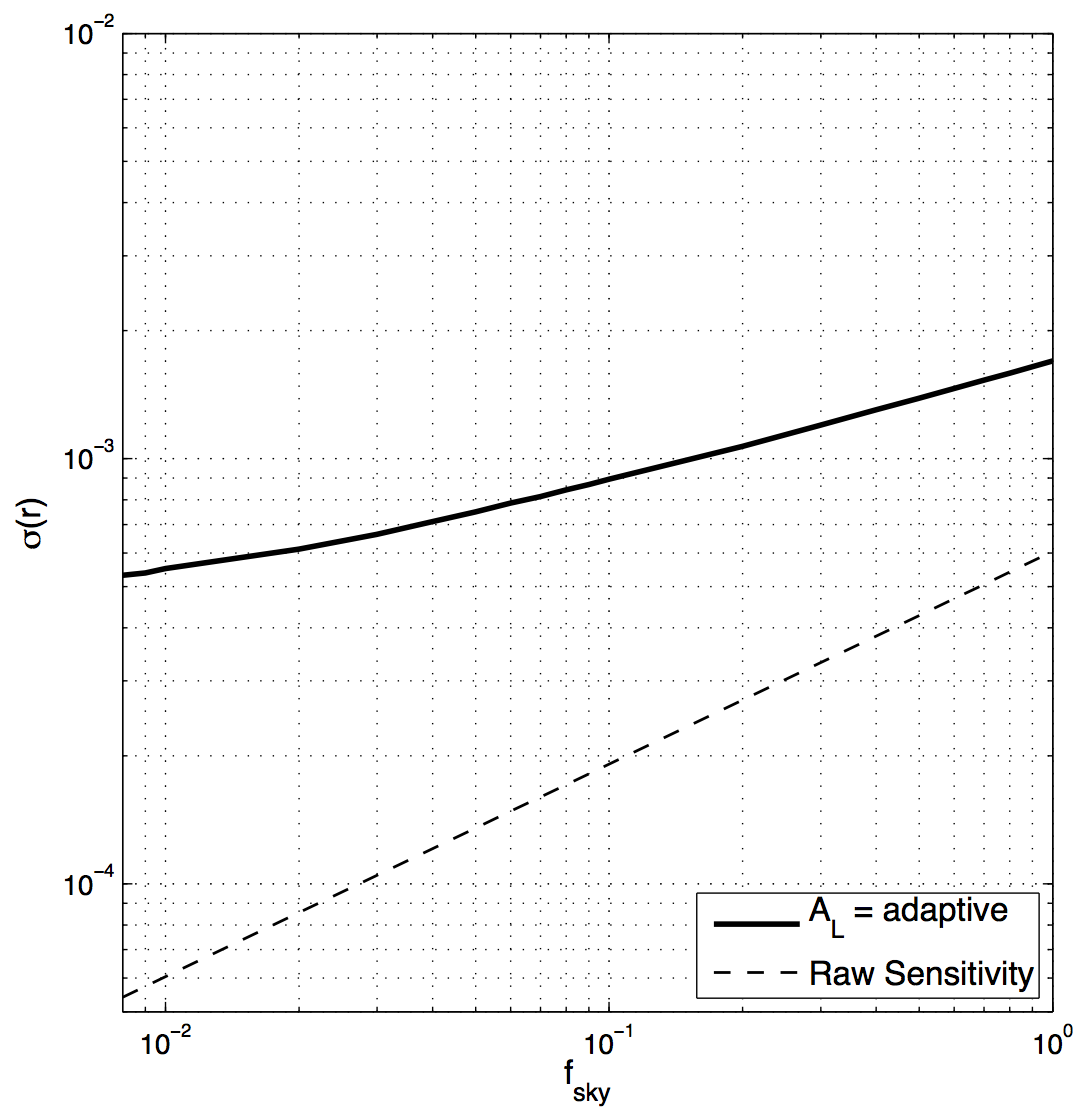
\includegraphics[width=0.49\textwidth]{Inflation/sigr_fsky_det1e6_r0.png}
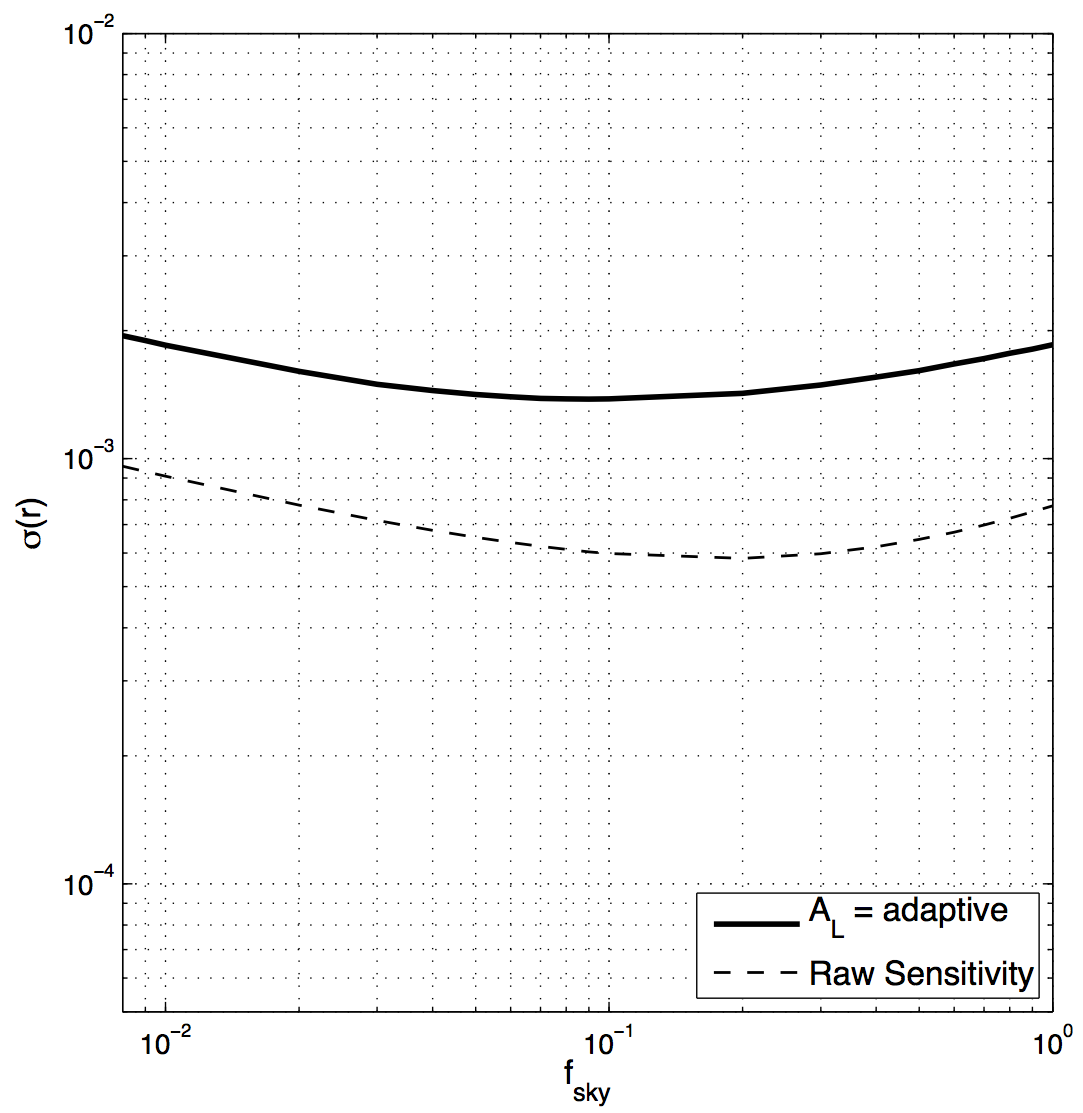
\includegraphics[width=0.49\textwidth]{Inflation/sigr_fsky_det1e6_r01.png}
\caption{Forecasted uncertainty on $r$, as a function of $f_{sky}$, for an
effort of $10^6$ detector-years (150 equivalent), assuming $r=0$ (left panel) 
and $r=0.01$ (right panel). The forecasting procedure is specifically targeted 
towards optimizing tensor-to-scalar parameter constraints in the presence of 
Galactic foregrounds and gravitational lensing of the CMB. The optimization 
assumes an amount of achieved delensing that varies with $f_{sky}$; temporary 
note: for a detailed description of the forecasting, please see: 
\href{http://users.physics.harvard.edu/~buza/20150331_fisher/}{this posting.}}
\label{fig_rforecast1}
\end{figure}

\begin{figure}[h]
\centering
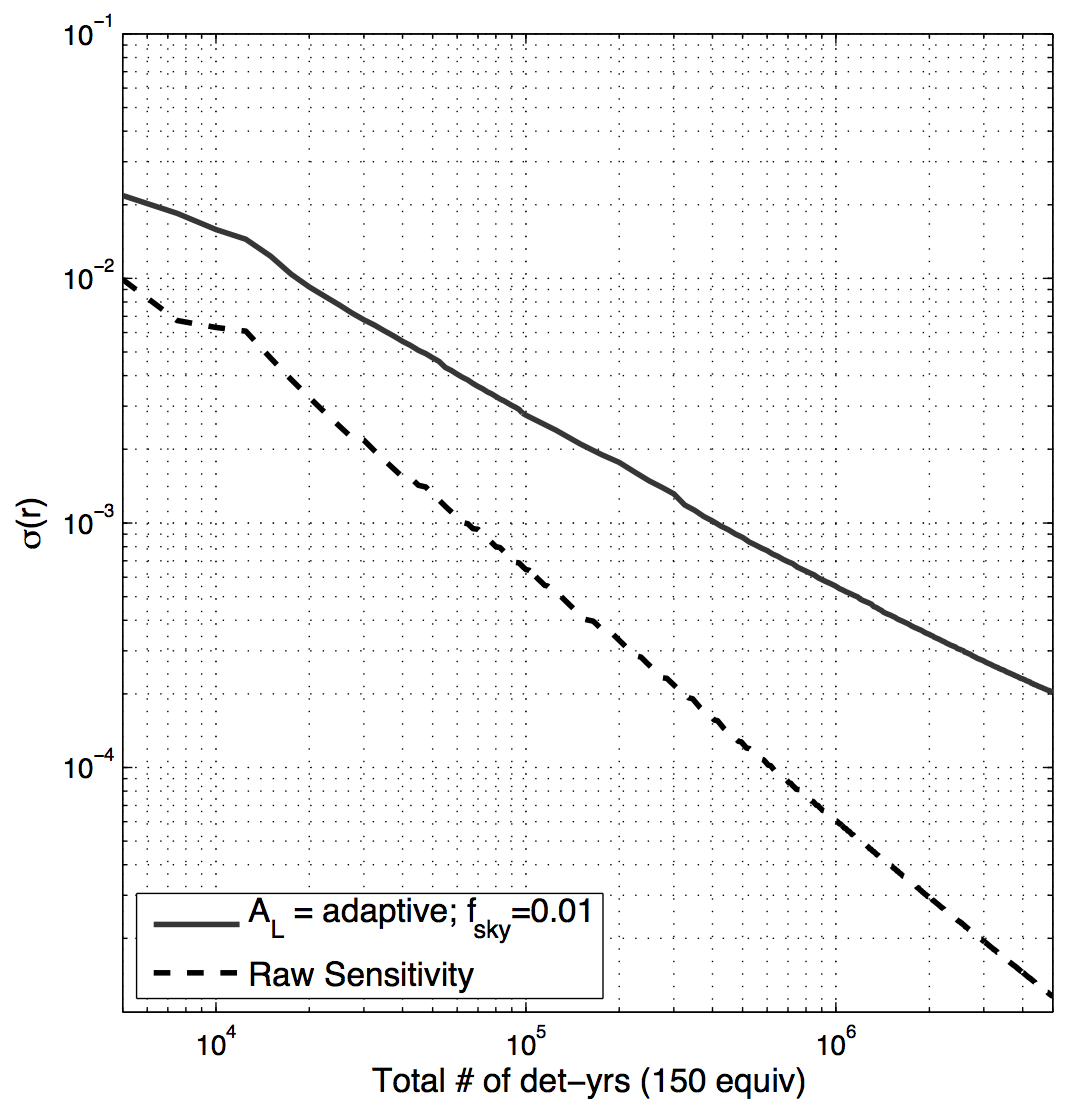
\includegraphics[width=0.49\textwidth]{Inflation/sigr_effort_r0.png}
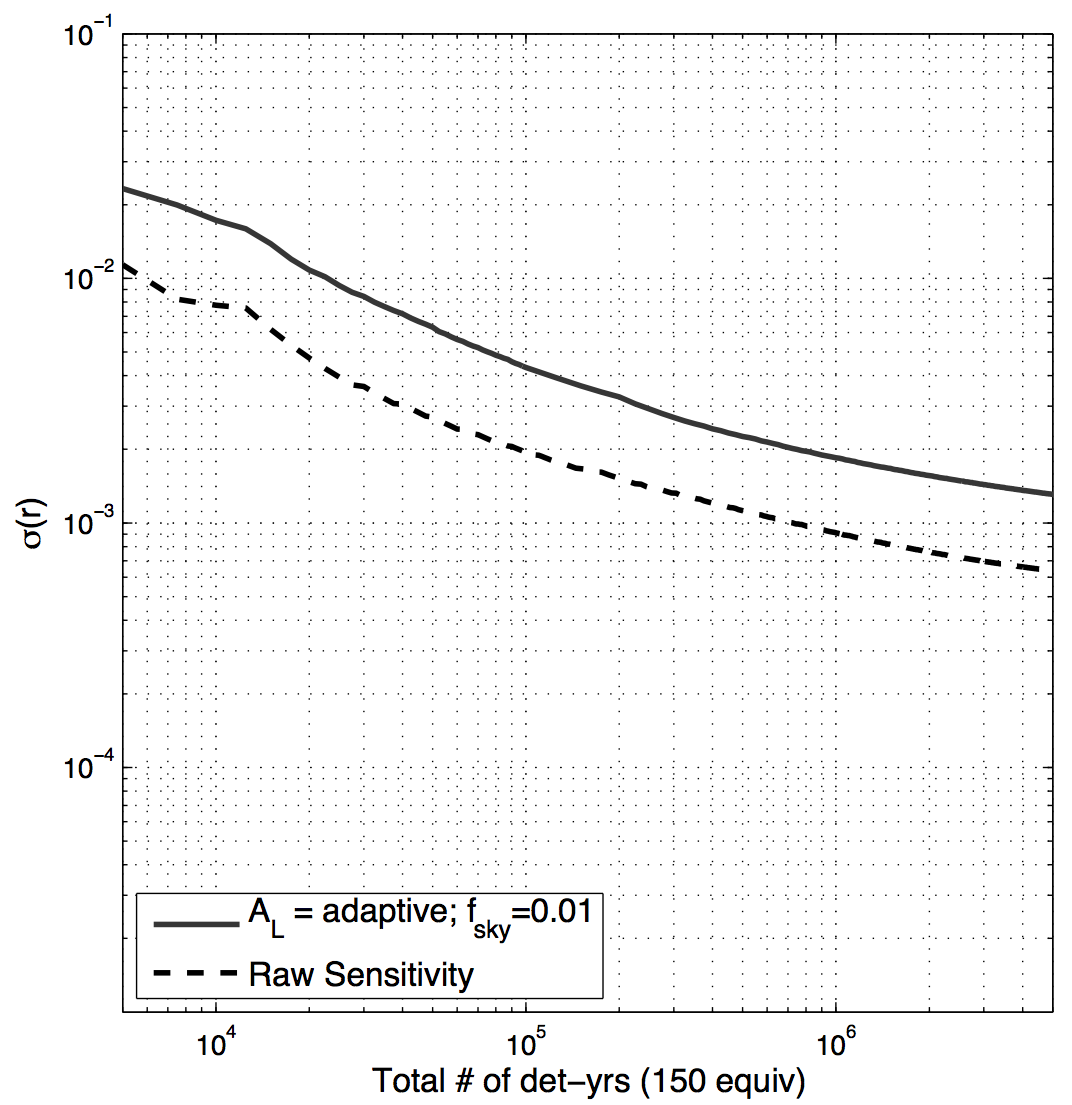
\includegraphics[width=0.49\textwidth]{Inflation/sigr_effort_r01.png}
\caption{Forecasted uncertainty on $r$, as a function of effort, for a fixed
$f_{sky}=0.01$, assuming $r=0$ (left panel) and $r=0.01$ (right panel).
The forecasting procedure is specifically targeted
towards optimizing tensor-to-scalar parameter constraints in the presence of 
Galactic foregrounds and gravitational lensing of the CMB. The optimization 
assumes an amount of achieved delensing that varies with $f_{sky}$; temporary 
note: for a detailed description of the forecasting, please see: 
\href{http://users.physics.harvard.edu/~buza/20150331_fisher/}{this posting.}  
}
\label{fig_rforecast2}
\end{figure}


\section{Improved constraints on primordial density perturbations}
\label{sec:scalar}
%CMB-S4 will either detect primordial gravitational waves or improve current constraints on the amplitude of their power spectrum by almost two orders of magnitude. In addition, CMB-S4 will significantly improve our knowledge of the statistical properties of primordial density perturbations. 
All current data are consistent with primordial density perturbations that are adiabatic, Gaussian, and nearly scale invariant. Because of its high angular resolution, CMB-S4 will significantly improve current constraints on the scale dependence of the primordial power spectrum of scalar perturbations, on departures from Gaussianity, and on departures from adiabatic perturbations. In fact, it will measure anisotropies in both the temperature and E-mode polarization of the CMB to cosmic variance over the entire range of multipoles that is not contaminated by unresolved foregrounds. As a consequence, it will place the strongest constraints achievable by any ground-based CMB experiment on all observables that benefit from the number of modes measured, such as the primordial power spectrum and higher order correlations.

\subsection{The power spectrum of primordial density perturbations}
%{\it The scalar spectral index}\\
The density perturbations are close to scale invariant but not exactly so. In the context of $\Lambda$CDM, {\it Planck} has measured the scalar spectral index to be $n_s=0.9677\pm0.0060$ and has established $n_s-1<0$ at more than $5\,\sigma$. CMB-S4 will improve current constraints on the spectral index by more than a factor of two to $\sigma(n_s)=0.0028$, and will provide valuable constraints on the space of inflationary models. 

%{\it Running of the scalar spectral index}\\
As mentioned in section~\ref{sec:upperLimits}, a measurement of the running of the scalar spectral index with a precision of a few parts in ten thousand would allow a measurement of $p$ in equation~(\ref{eq:nsassump}), or equivalently $\mathcal{N}_\star$. This precision cannot be achieved with CMB-S4, but with a precision of one part in a thousand, it will test the idea that the lack of power on large angular scales might be explained by scale dependence of the spectral index~\cite{Meerburg:2014bpa}.  

%{\it Oscillations in the primordial power spectrum}\\
Models of inflation that achieve super-Planckian inflaton displacements from repeated circuits of a sub-Planckian fundamental period may give rise to oscillatory features in the spectrum of primordial perturbations. The features may arise either from instanton effects or from periodic bursts of particle or string production. A search for such features is well motivated even though the amplitude is model-dependent and may be undetectably small. A detection would provide clues about the microscopic origin of the inflaton, the absence of a detection can constrain the parameters space of these models in interesting ways. CMB-S4 would tighten the constraints on the amplitude of features in the primordial power spectrum by a factor of three. 

Other physical effects during inflation can lead to small features in the observed power spectrum, e.g by changing the equation of state during inflation \cite{}. Because of the stringent constraints on the minimum number of E-folds, such modifications can not last very long in order not to end inflation and associated features only affect a small range of scales. It is therefore unlikely that CMB-S4 will significanty improve constraints on these type of features unless they are on very small scales. 
 
\subsection{Higher order correlations}
Any detection of departures from Gaussianity would shed light on the interactions either of the inflaton with itself or between the inflaton and other degrees of freedom. From the discussion of various scenarios to produce primordial B-modes, it is also a common theme that constraints on non-Gaussianity significantly cut into the model space of proposals to produce a B-mode signal of observable strength other than the standard inflationary signal. 

The lowest order correlation function that encodes departures from Gaussianity is the $3pt$-function
\begin{equation}
\langle\zeta(\vec{k}_1)\zeta(\vec{k}_2)\zeta(\vec{k}_3)\rangle=(2\pi)^3\delta(\vec{k}_1+\vec{k}_2+\vec{k}_3)B(\vec{k}_1,\vec{k}_2,\vec{k}_3)\,,
\end{equation}
where the delta function comes from translation invariance. Many scenarios invariance under rotations and translations guarantee that the bispectrum $B(k_1,k_2,k_3)$ only depends on the magnitudes $k_1$, $k_2$, and $k_3$. A model independent search for the bispectrum, or equivalently the angular bispectrum $b_{\ell_1\ell_2\ell_3}$, is not computationally tractable, and in practice searches place constraints on the amplitudes $f_{\rm NL}$ of certain theoretically motivated functional forms, or shapes.

Perhaps of special interest for CMB-S4 are non-Gaussian signatures that would be expected in models of large field inflation. For example, in models in which the inflaton is an axion, there is only an approximate discrete shift symmetry. In that case instanton contributions to the potential and periodic bursts of particle or string production naturally lead to periodic features in the bispectrum. If moduli in the underlying string constructions do not evolve appreciably, instanton contributions lead to oscillations with a constant amplitude in the logarithm of $k$. In general, moduli evolve during inflation and cause a drift in the frequency and a scale-dependent amplitude~\cite{Flauger:2014ana}. At present, these shapes have not yet been constrained systematically. Often these contributions will lead to counter-parts in the power spectrum and are expected to be detected there first~\cite{Behbahani:2011it}, but this need not be the case~\cite{Behbahani:2012be}. A first attempt has been made~\cite{Ade:2015ava} to look for resonant and local features in the bispectrum and a more dedicated analysis is underway. Since features in the power spectrum and the bispectrum generally contain correlated parameters \cite{Achucarro:2010da,NonBDBispectrum2009,nonBDbispectrum2015,Flauger:2010ja} statistical methods have been developed to use the power of both the power spectrum and the bispectrum to further constrain models space \cite{Meerburg2015b,Moritz2016,Fergusson:2014hya}. Signatures of higher order massive spin fields \cite{Arkani-Hamed:2015bza,Chen:2015lza} would also lead to a bispectrum with decaying features, which will not be present in the power spectrum.  So a search for these more general shapes is well motivated. Using both $T$ and $E$-mode polarization, CMB-S4 will improve constraints by about of two compared to {\it Planck} as we will show in the next section. Bispectra containing at least one $B$ mode, will generally be much better constrained (currently there is no bound on such correlation functions) and will benefit from CMB-S4. We will consider two examples in the next section. 

More generally, one can divide the space of non-Gaussian inflationary models into those whose signals either (1) indicate fluctuations in degrees of freedom other than the inflaton, or (2) indicate non-trivial self-interactions of the effective inflaton fluctuation. Given the forecasted improvements from CMB-S4 over the {\it Planck}, it is unlikely that this instrument would uncover strong evidence of non-Gaussianity. However, since the {\it Planck} constraints have not ruled out $f_{\rm NL}\sim\mathcal{O}(1)$, even a hint of non-Gaussianity would be extremely interesting. Here we briefly review the physics in the two cases.

A detection of the widely studied local shape would have far reaching theoretical implications. A detection of this shape would rule out all models of single clock inflation \cite{Creminelli:2004yq}. In addition, such a signal would open the door to significant cosmic variance on all scales from coupling of fluctuations within our observed volume to any super-Hubble modes \cite{Nelson:2012sb,LoVerde:2013xka,Nurmi:2013xv}. Indeed, there would be room for a significant shift between the observed amplitude of scalar fluctuations (and so the observed $r$) and the mean value of fluctuations on much larger scales \cite{Bonga:2015urq}. Any scenario that predicts local non-Gaussianity together with fluctuations on scales much larger than our observed volume predicts a probability distribution for our observed $f_{\rm NL}^{\rm local}$, but many well-motivated scenarios also predict a small mean value. These include the simplest modulated reheating scenario \cite{Zaldarriaga:2003my} and ekpyrotic cosmology \cite{Lehners:2009ja}, both of which predict mean values of $f_{\rm NL}^{\rm local}\sim5$. 
Currently the strongest constraints on the local shape come from the {\it Planck} 2015 temperature and polarization analysis which finds $f_{\rm NL}^{\rm local} = 0.8 \pm 5.0$~\cite{Ade:2015ava}. A noise-free cosmic variance limited CMB experiment is expected to produce constraints on $f_{\rm NL}^{\rm local}$ with 1$\sigma$ error bars of about 3 \cite{Komatsu:2001rj}. Therefore the improvement expected of CMB-S4 over current limits is slightly less than a factor of two. This is not sufficient to reach the interesting theoretical threshold around $|f_{\rm NL}^{\rm local}|\lesssim 1$~\cite{Alvarez:2014vva}, but will still reduce the space of viable models or hint at a detection. CMB-S4 could, for example, provide hints for the mean level of non-Gaussianity expected from modulated reheating scenario or ekpyrotic cosmology at roughly $2\,\sigma$. The simplest curvaton scenario, which predicts $f_{\rm NL} = -5/4$ \cite{Lyth:2001nq}, will unfortunately be out of reach. Large-scale structure surveys (eg., \cite{Dore:2014cca}) may eventually achieve constraints $\sigma_{f_{\rm NL}}\sim\mathcal{O}(1)$. Those observations of the inhomogeneities in the late universe would be very complementary to the results of CMB-S4.

Equilateral and orthogonal shapes shapes arise in scenarios where the scalar perturbations sourced by inflaton fluctuations have non-trivial self interactions, and indicate an additional scale of particle physics, $M_{c_s}$ between $H$ and $M_p$. The amplitude of the non-Gaussianity typically scales as $(H/M_{c_s})^2$. Current constraints on the equilateral and orthogonal shapes are $f_{\rm NL}^{\rm equil} = -4 \pm 43$ and $f_{\rm NL}^{\rm ortho} = -26 \pm 21$, both (68\% CL)~\cite{Ade:2015ava}, which translates into $M_{c_s}>\mathcal{O}(10)H$. The improvements from CMB-S4 would further tighten existing constraints on the speed of sound during inflation and the strong coupling scale in single-clock models of inflation. In addition, the tighter constraints on the equilateral shape would constrain scenarios with secondary production of gravitational waves.

\subsection{Forecasts}

\begin{figure}[htbp!]
\centering
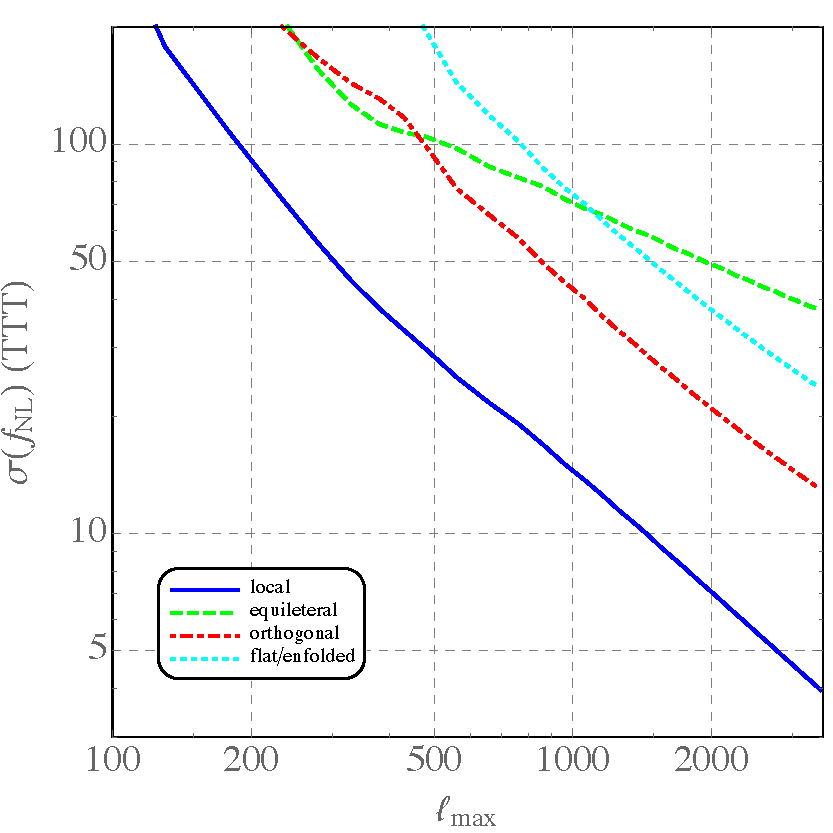
\includegraphics[width=0.43\textwidth]{Inflation/DeltaFNL_TTT}
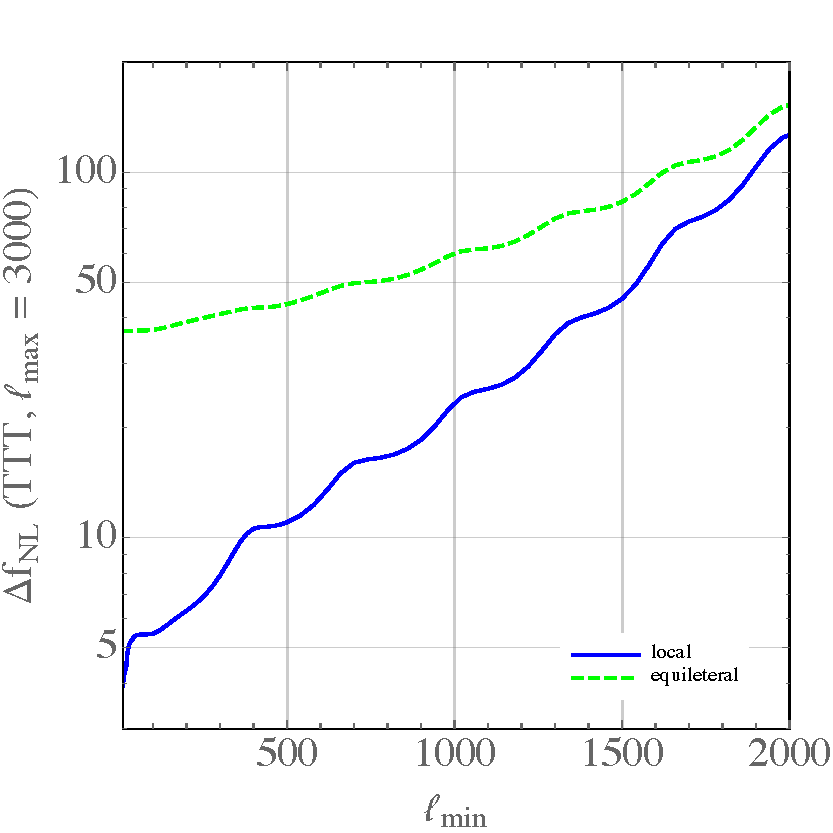
\includegraphics[width=0.43\textwidth]{Inflation/DeltaFNL_TTT_lmin}
\caption{Left: forecasts on the constraining power of CMB-S4 combined with {\it Planck} on 3 different types of non-Gaussianities as a function of $\ell_{\rm max}$ using $T$ and $E$ modes. Right: Sensitivity of local type non-Gaussianities as a function of the minimum multipole. The local type non-Gaussianity benefits from having the lowest multipoles, while the other standard shapes saturate to a constant at low $\ell_{\rm min}$ (not shown, see Tab.~\ref{tab:fnl_forecast}). The above plot was generated using $f_{\rm sky} = 0.4$, $T$-noise = 1 $\mu$K-' and $E$-noise = $\sqrt{2}$ $\mu$K-' and a beam of $1$' and $\ell_{\rm min} = 30$ combined with {\it Planck} Blue Book values in the range $2\leq \ell_{\rm min} \leq 30$.}
\label{fig_fnlforecast}
\end{figure}

We forecast the constraints on non-Gaussianities from CMB-S4. We consider the most well motivated shapes; local, equilateral, orthogonal and enfolded. 
In Fig.~\ref{fig_fnlforecast} we show the constraints as a function of the maximum multipole on the left using the following configuration $f_{\rm sky} = 0.4$, $T$-noise = 1 $\mu$K-' and $E$-noise = $\sqrt{2}$ $\mu$K-' and a beam of $1$' and $\ell_{\rm min} = 30$. Local type non-Gaussianities benefit from large scales, and as much as $40\%$ of the signal is lost if these modes are not available as cab be seen in Fig.~\ref{fig_fnlforecast} on the right. Ideally, large scale information from Planck \cite{Ade:2015ava} should be included to put the best constraints on non-Gaussianities. Including Planck low $\ell$ (using $f_{\rm sky} = 0.75$ \cite{Ade:2015ava} to determine the noise level, and $f_{\rm sky}=0.4$ for the maximal overlap) we can improve the forecasted bounds on local type non-Gaussianities by almost a factor of 2. Equilateral, enfolded and orthogonal non-Gaussianities are not affected by not including the lowest multipoles. We summerize the results in Tab.~\ref{tab:fnl_forecast}. Note that our forecast, using Planck Blue Book\footnote{\url{http://www.rssd.esa.int/SA/PLANCK/docs/Bluebook-ESA-SCI(2005)1_V2.pdf}} values, deviate slightly from the actual bounds on non-Gaussianities obtained in Ref.~\cite{Ade:2015ava}. The expected factor of improvement over {\it Planck}-only is somewhere between 1.7 and 1.8 for all shapes considered. Information saturates beyond $\ell_{\rm max} = 5000$ for all shapes for an experiment with $1$' beam. 

% Requires the booktabs if the memoir class is not being used
\begin{table*}[t]\label{tab:fnl_forecast}
  \begin{center}
    \begin{tabular}{ | c || c | c | c | c |}
      \hline
      Type & Planck & CMB-S4 & CMB-S4 + low $\ell$ Planck & rel. improvement \\ \hline \hline
      local & $\sigma(f_{\rm NL}) = 3.1$ & $\sigma(f_{\rm NL}) = 2.8$ &  $\sigma(f_{\rm NL}) = 1.8$ & 1.7\\ \hline 
      equilateral &  $\sigma(f_{\rm NL}) = 32.1$ & $\sigma(f_{\rm NL}) = 18.8$ &  $\sigma(f_{\rm NL}) = 18.8$ & 1.7\\ \hline 
      orthogonal &  $\sigma(f_{\rm NL}) = 15.4$ & $\sigma(f_{\rm NL}) = 8.7$ &  $\sigma(f_{\rm NL}) = 8.7$ & 1.8\\ \hline 
      flat &  $\sigma(f_{\rm NL}) = 26.1$ & $\sigma(f_{\rm NL}) = 15.2$ &  $\sigma(f_{\rm NL}) = 15.2$ & 1.7\\ \hline 
    \end{tabular}
  \end{center}
  \caption{Forecasted constraints on several well motivated non-Gaussian shapes using $T$ and $E$ modes. {\it Planck} forecast is based on Blue Book values, with $f_{\rm sky} = 0.75$. The table shows we need to include low $\ell$ information from {\it Planck} for local type non-Gaussianities.}
  \label{default}
\end{table*}

\begin{figure}[htbp!]
\centering
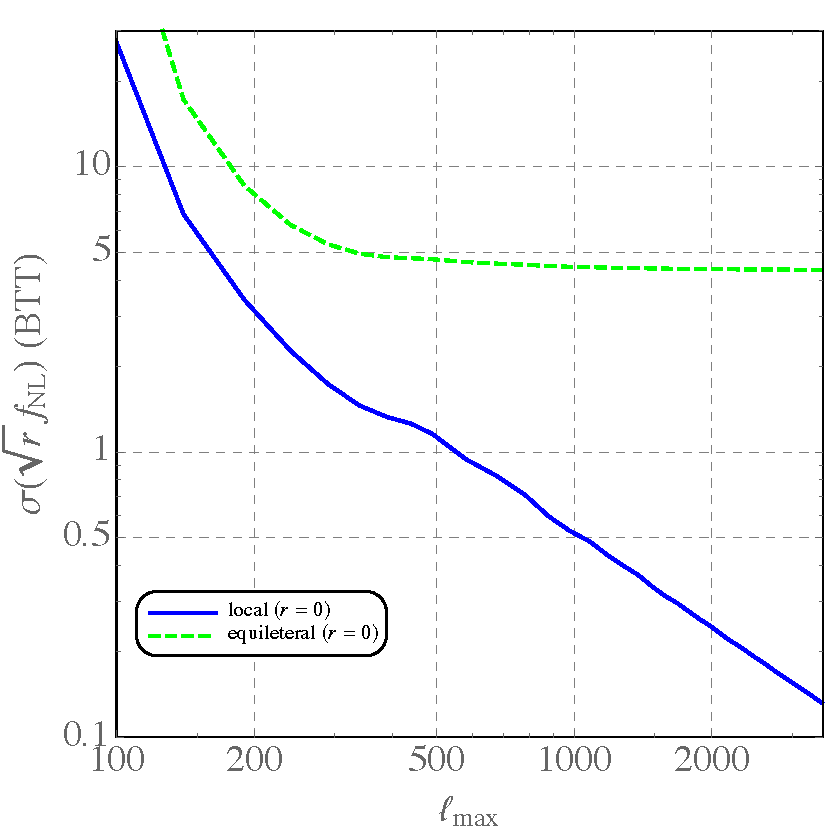
\includegraphics[width=0.45\textwidth]{Inflation/DeltaFNL_BTT_no_r}
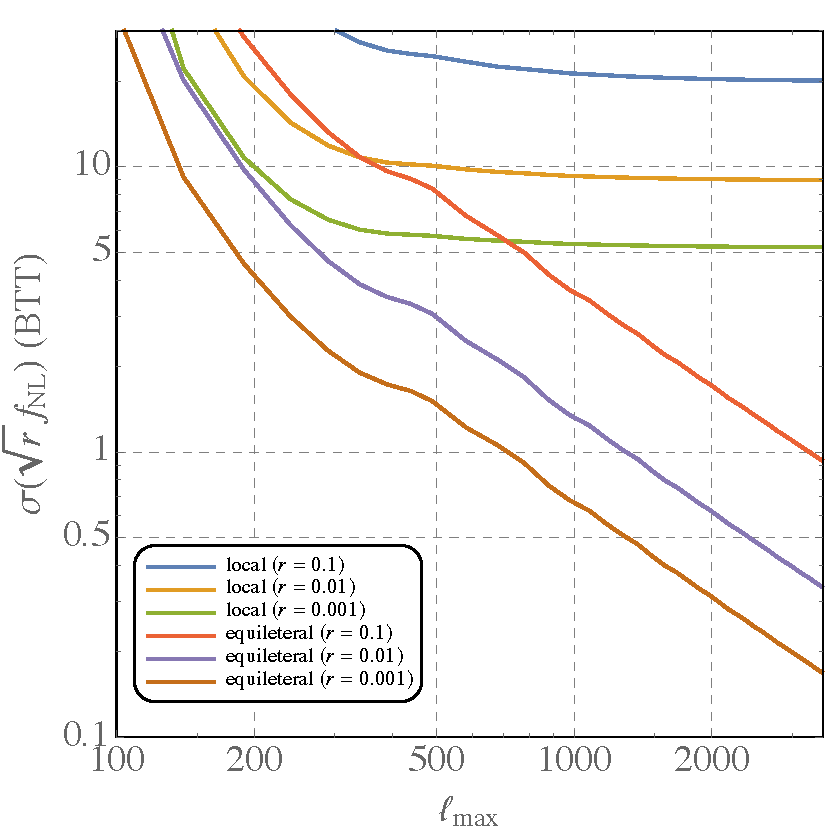
\includegraphics[width=0.45\textwidth]{Inflation/DeltaFNL_BTT_with_r}
\caption{Left: Noise dominated $B$ modes. Forecasts on the constraining power of CMB-S4 on two types of $\langle h \zeta \zeta\rangle$ non-Gaussianities as a function of $\ell_{\rm max}$ using $\langle BTT\rangle$. Right: the effect of cosmic variance in $B$.  }
\label{fig_fnlforecastBTT}
\end{figure}

Next, we determine the improvements as function of a fixed effort with $f_{\rm sky} = 0.4$ corresponding to noise of 1 $\mu$K-arcmin.  {\color{blue} To do this weekend/early next week}. 

Correlators including at least one $B$ mode will benefit from the improved sensitivity of $B$ modes significantly. We define \cite{Meerburg2016}
\begin{equation}
\langle \zeta(\vec{k}_1)\zeta(\vec{k}_2)h^{\pm}(\vec{k}_3) \rangle = (2\pi)^3  \delta^{(3)} \left(\sum_{n=1}^3\vec{k}_n\right) \mathcal{B}(k_1,k_2,k_3) e_{ab}^{\mp}(\vec{k}_3)\hat{k}_1^a \hat{k}_2^b, 
\end{equation}
with 
\begin{equation}
\mathcal{B}(k_1,k_2,k_3)= 16 \pi^4 A_s^2 \sqrt{r}f_\mathrm{NL}^{h\zeta\zeta} F(k_1,k_2,k_3)
\end{equation}
and $e_{ab}^{\mp}$ the transverse traceless polarization tensor. 
In the simplest model of inflation $f^{h \zeta \zeta}_{\rm NL} = \sqrt{r}/16$ \cite{Maldacena:2002vr,Maldacena:2011nz} which realistically is undetectable. As mentioned before in Sec.~\ref{subsubsec:Interactions}, a measurement if this correlation would be an immediate indication of some deviation from the simple inflationary paradigm and as such would provide valuable information. The coupling above can be constrained using any type of correlation that contains one $B$ mode, e.g. $\langle BTT \rangle$ or $\langle BEE\rangle$. For $F$ we use local and equilateral shaped triangles and forecast the constraint on the amplitude in Fig.~\ref{fig_fnlforecastBTT} for $\langle BTT\rangle$. We anticipate similar constraints for $\langle BTE\rangle $ and $\langle BEE\rangle$. 


\begin{table*}[t]\label{tab:fnl_forecast2}
  \begin{center}
    \begin{tabular}{ | c || c | c | c | c |}
      \hline
      Type & Planck & CMB-S4 & rel. improvement  \\ \hline \hline
      local & $\sigma(\sqrt{r}f_{\rm NL}) = 15.2$ & $\sigma(\sqrt{r}f_{\rm NL}) = 0.3$ & 50.7\\ \hline 
      equilateral &  $\sigma(\sqrt{r}f_{\rm NL}) = 200.5$ & $\sigma(\sqrt{r}f_{\rm NL}) = 7.4$ & 27.1\\ \hline 
      local ($r = 0.01$) & $\sigma(\sqrt{r}f_{\rm NL}) = 15.2$ & $\sigma(\sqrt{r}f_{\rm NL}) = 0.7$ & 25.3\\ \hline 
      equilateral ($r = 0.01$) &  $\sigma(\sqrt{r}f_{\rm NL}) = 200.8$ & $\sigma(\sqrt{r}f_{\rm NL}) = 14.7$ & 13.7\\ \hline 
    \end{tabular}
  \end{center}
  \caption{Forecasted constraints on local and equilateral shapes sourced by primordial and equilateral correlations of the form $\langle h \zeta\zeta \rangle$ constrained through $\langle BTT \rangle$. {\it Planck} forecast is based on Blue Book values, with $f_{\rm sky} = 0.75$. Constraints were derived using the flat-sky approximation as in Ref.~\cite{Meerburg2016} with $\ell_{\rm min} = 30$ with no cosmic variance in $B$.  We expect similar constraints from $\langle BEE \rangle$ and $\langle BTE \rangle$. For $r = 0.01$ {\it Planck} is still noise dominated, while CMB-S4 is cosmic variance dominated. }
  \label{default}
\end{table*}



\begin{figure}[htbp!]
\centering
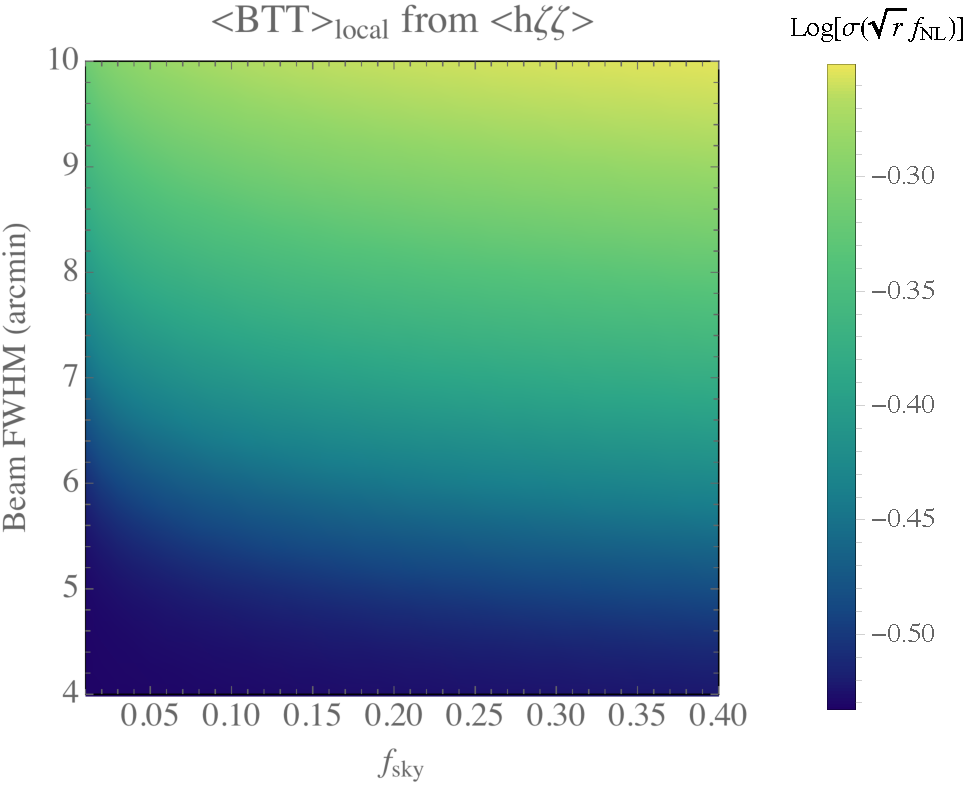
\includegraphics[width=0.48\textwidth]{Inflation/FixedEffortBTTlocal}
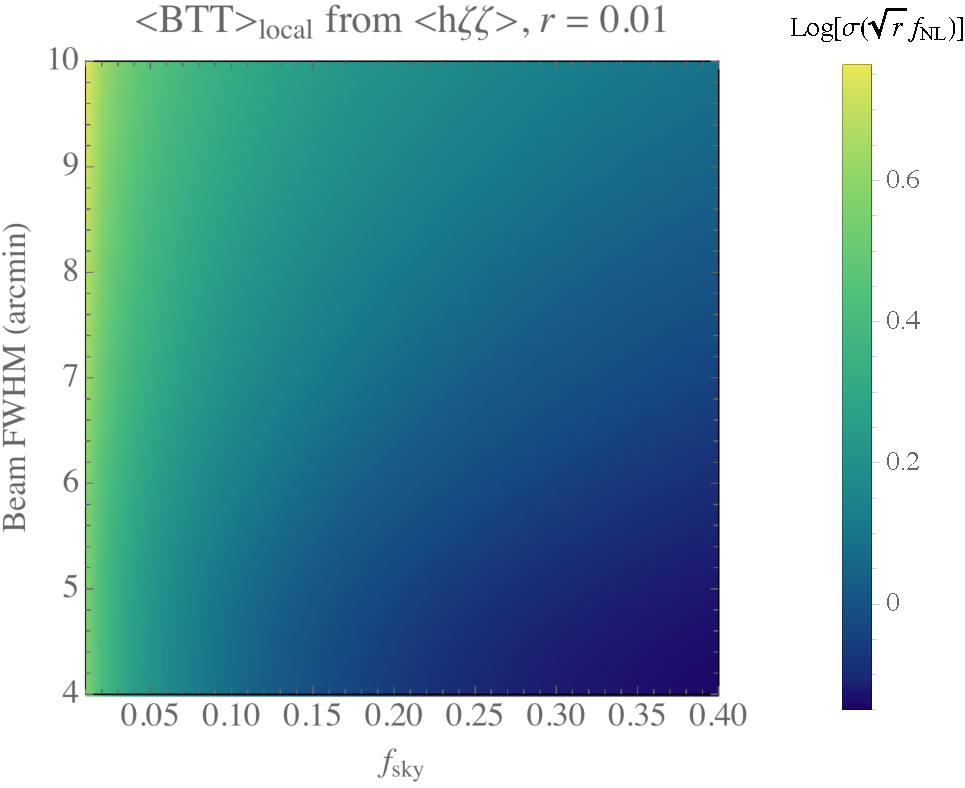
\includegraphics[width=0.48\textwidth]{Inflation/FixedEffortBTTlocalr}
\caption{Left: Fixed effort density plot for local type $BTT$. Left, the effect of beam and $f_{\rm sky}$ variation in noise dominated $B$ mode. $f_{\rm sky}$ has very little effect, as it is cancelled by the $f_{\rm sky}$ associated with the masking of the total map. Right: adding a signal changes this picture, since the cancellation no longer happens for $r > 0.001$ (i.e. when CMB-S4 becomes cosmic variance limited). A larger sky fraction benefits cosmic variance limited $\langle BTT\rangle$. }
\label{fig_BTTlocalfixedeffort}
\end{figure}




We consider two scenarios; one in which the $B$ modes are noise dominated and one in which they are cosmic variance limited by a future detection of $r$. For a local shape primordial bispectrum the error decreases as you decrease the beam. The signal is dominated by large angle $B$ modes correlated with small angle $T$ modes as was pointed out in \cite{Meerburg2016}. An equilateral component from the $\langle BTT\rangle$ correlation function suffers from the decaying tensor modes, which are negligible for $\ell_B > 500$. After this, no equilateral triangles can be constructed and the error saturates. The effect is that equilateral type non-Gaussianities are almost insensitive to beam size. 

On the right we show what happens when $B$ gets a primordial component; the take away message is that only if $r < 0.001$  CMB-S4 noise dominates cosmic variance. We compare the potential constraining power of {\it Planck} to that of CMB-S4 in Tab.~\ref{tab:fnl_forecast2}. 

In addition we consider fixed effort. We show the results in Fig.~\ref{fig_BTTlocalfixedeffort} and \ref{fig_BTTequilfixedeffort}. We find that $BTT$ is practically insensitive to $f_{\rm sky}$ as long as $B$ modes are noise dominated. For $r = 0.001$ and above a larger sky fraction helps constrain $\langle BTT \rangle$. 

\begin{figure}[htbp!]
\centering
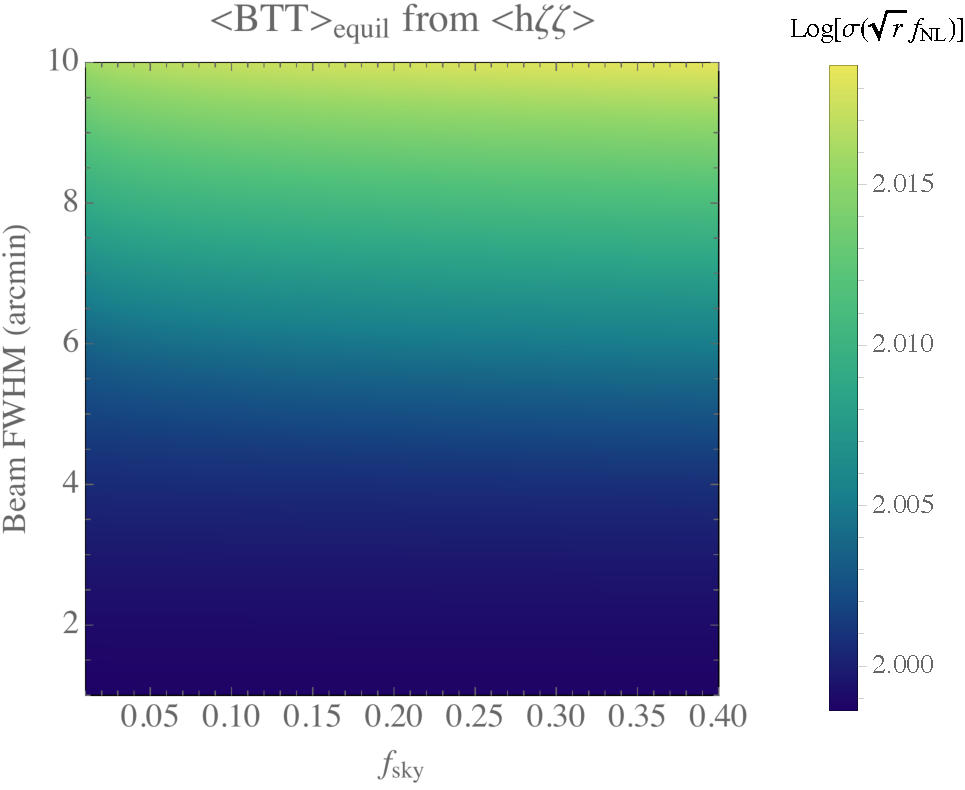
\includegraphics[width=0.48\textwidth]{Inflation/FixedEffortBTTequil}
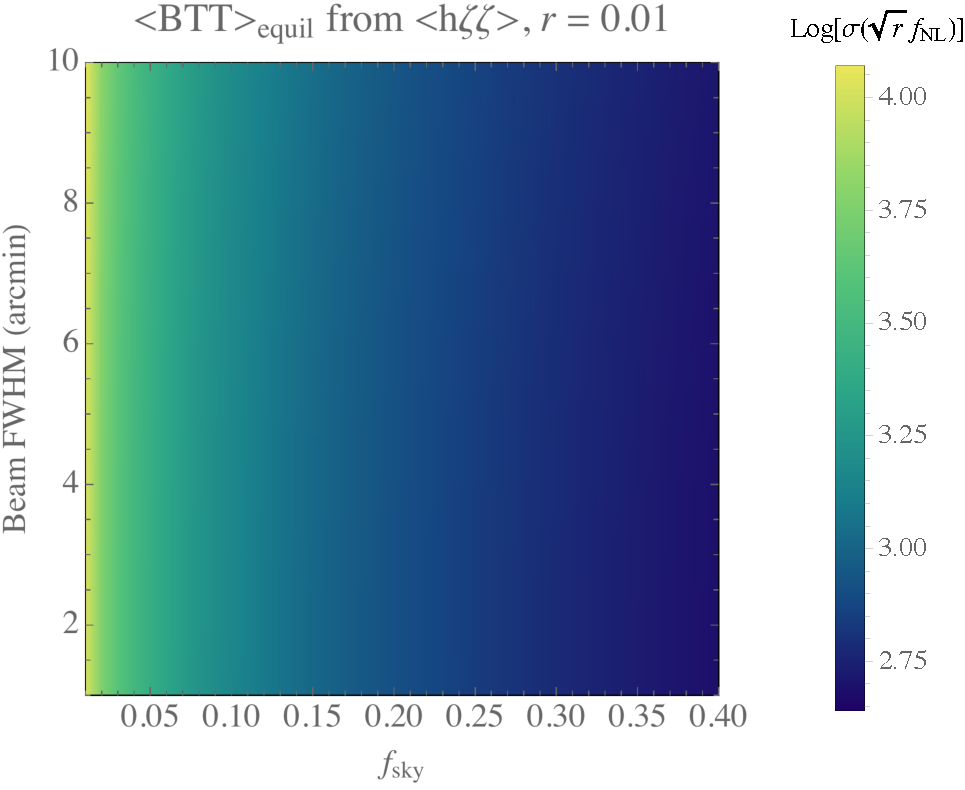
\includegraphics[width=0.48\textwidth]{Inflation/FixedEffortBTTequilr}
\caption{Left: Fixed effort density plot for equilateral type $BTT$. Similar to local type bispectra, a larger sky fraction benefits cosmic variance limited $\langle BTT\rangle$. }
\label{fig_BTTequilfixedeffort}
\end{figure}
%In models with a single clock, the symmetry breaking pattern underlying inflation guarantees that the fluctuations are governed by the action
%\begin{equation}
%S=\int\,d^4 x \sqrt{-g}\left[-\frac{M_p^2 \dot{H}}{c_s^2}\left(\dot{\pi}^2-c_s^2\frac{(\partial_i\pi)^2}{a^2}\right)+M_p^2 \dot{H}\left(1-\frac{1}{c_s^2}\right)\left(\dot\pi^3-\dot\pi\frac{(\partial_i\pi)^2}{a^2}\right)+M_3^4\dot\pi^3+\dots\right]\,,
%\end{equation}
%where at leading order $\zeta=H\pi$ and the omissions represent terms higher order in fields, derivatives, or both. In the presence of an approximate continuous shift symmetry, the coefficients in this action are approximately constant in time and there are only two linearly independent shapes. 
%Current constraints on the equilateral and orthogonal shapes are $f_{\rm NL}^{\rm equil} = -4 \pm 43$ and $f_{\rm NL}^{\rm ortho} = -26 \pm 21$, both (68\% CL)~\cite{Ade:2015ava}. Because of its high angular resolution, CMB-S4 can improve these constraints by about a factor two which would further tighten existing constraints on the speed of sound during inflation and the strong coupling scale in single-clock models of inflation. In addition, the tighter constraints on the equilateral shape would constrain scenarios with secondary production of gravitational waves.

{\color{blue} Any one care to work this out more:} 
Higher order statistics encode further information about particle content and interactions. The relative amplitude of certain limits of the trispectrum (the momentum space 4-point function) and of the trispectrum can also reveal whether there may be multiple sources contributing to the primordial fluctuations (and both may be different from the fluctuations of the inflaton). {\bf more...}


%In the modulated reheating scenario, the field which drives inflation $\phi$ decays to the particles of the standard model with a rate $\gamma$ which is determined by the value of a second field $\sigma$ which remains light throughout inflation. The quantum fluctuations in $\sigma$ result in a spatially modulated reheating surface resulting in the curvature perturbations that we observe in the CMB and large scale structure. The process by which the fluctuations in the light field are converted into curvature fluctuations naturally results in local non-Gaussianity given by $f_{\rm NL} = 5(1-\Gamma \Gamma^{\prime\prime}/\Gamma^{\prime2})$, where this formula holds in the case that $\phi$ oscillates about a quadratic minimum after inflation and the fluctuations in $\phi$ make a negligible contribution to the observed power spectrum.

%This can be contrasted with the simplest curvaton scenario, where a scalar field $\sigma$ which remains light during inflation comes to dominate the energy density of the universe after the field which drives inflation $\phi$ decays. The fluctuations in the energy density of $\sigma$ then determine the curvature perturbations that are observed today. The local non-Gaussianity in this simple model is predicted to be $f_{\rm NL} = -5/4$ \cite{Lyth:2001nq}, which is unfortunately a few times smaller than the expected error bar from CMB Stage-IV.

%In the absence of a detection, however, it is important to ask what can be learned from improved constraints on $f_{\rm NL}$. Though not firm, nor entirely robustly defined, it can be argued that a natural theoretical threshold where qualitatively new general conclusions about the physics of the early universe can be drawn would come from constraints on $f_{\rm NL}<\mathcal{O}(1)$, see for example [1412.4671] for a detailed discussion. In order to achieve this level of constraint, it seems necessary to move beyond the cosmic microwave background to study other data sets, such as large scale structure. Despite the fact that CMB Stage-IV is not expected to reach this threshold, it is worth asking what can be gleaned from an improved constraint on $f_{\rm NL}$ from the CMB.

\section{Isocurvature}
Measurements of CMB temperature/polarization power spectra indicate that the primordial initial conditions are adiabatic, that is, spatial entropy fluctuations vanish:
\begin{align}
S_{i \gamma}\equiv \frac{\delta n_{i}}{n_{i}}-\frac{\delta n_{\gamma}}{n_{\gamma}} =0.\end{align} The species label $i$ can denote baryons, cold dark matter (CDM), or neutrinos. Number densities are denoted by $n_{i}$ and perturbations in them by $\delta n_{i}$.

Adiabatic perturbations are produced in models where the initial perturbations in all species are seeded by the inflaton. If fluctuations are also sourced by a second field, the initial conditions are a mixture of adiabatic and entropy (a.k.a isocurvature) perturbations, for which $S_{i\gamma}\neq 0$. These initial conditions determine the acoustic peak structure and large-scale amplitude of CMB anisotropies, as well as large-scale structure statistics \cite{Bond:1984fp,Kodama:1986fg,Kodama:1986ud,Hu:1994jd,Moodley:2004nz,Bean:2006qz}. Observations can thus probe the number of fields during inflation. 
\label{sec:isosec}
Each species can carry isocurvature perturbations in its density (e.g. Refs~\cite{Bucher:1999re,Bucher:2004an,Moodley:2004nz}).\footnote{Neutrinos can also carry velocity isocurvature, but this mode is not well motivated in inflationary models.} Indeed, the modes of the perturbation evolution equations correspond to adiabatic, CDM density isocurvature (CDI), baryon density isocurvature (BDI), neutrino density isocurvature (NDI), and neutrino velocity isocurvature (NVI) initial conditions. 

\begin{figure*}[htbp!]
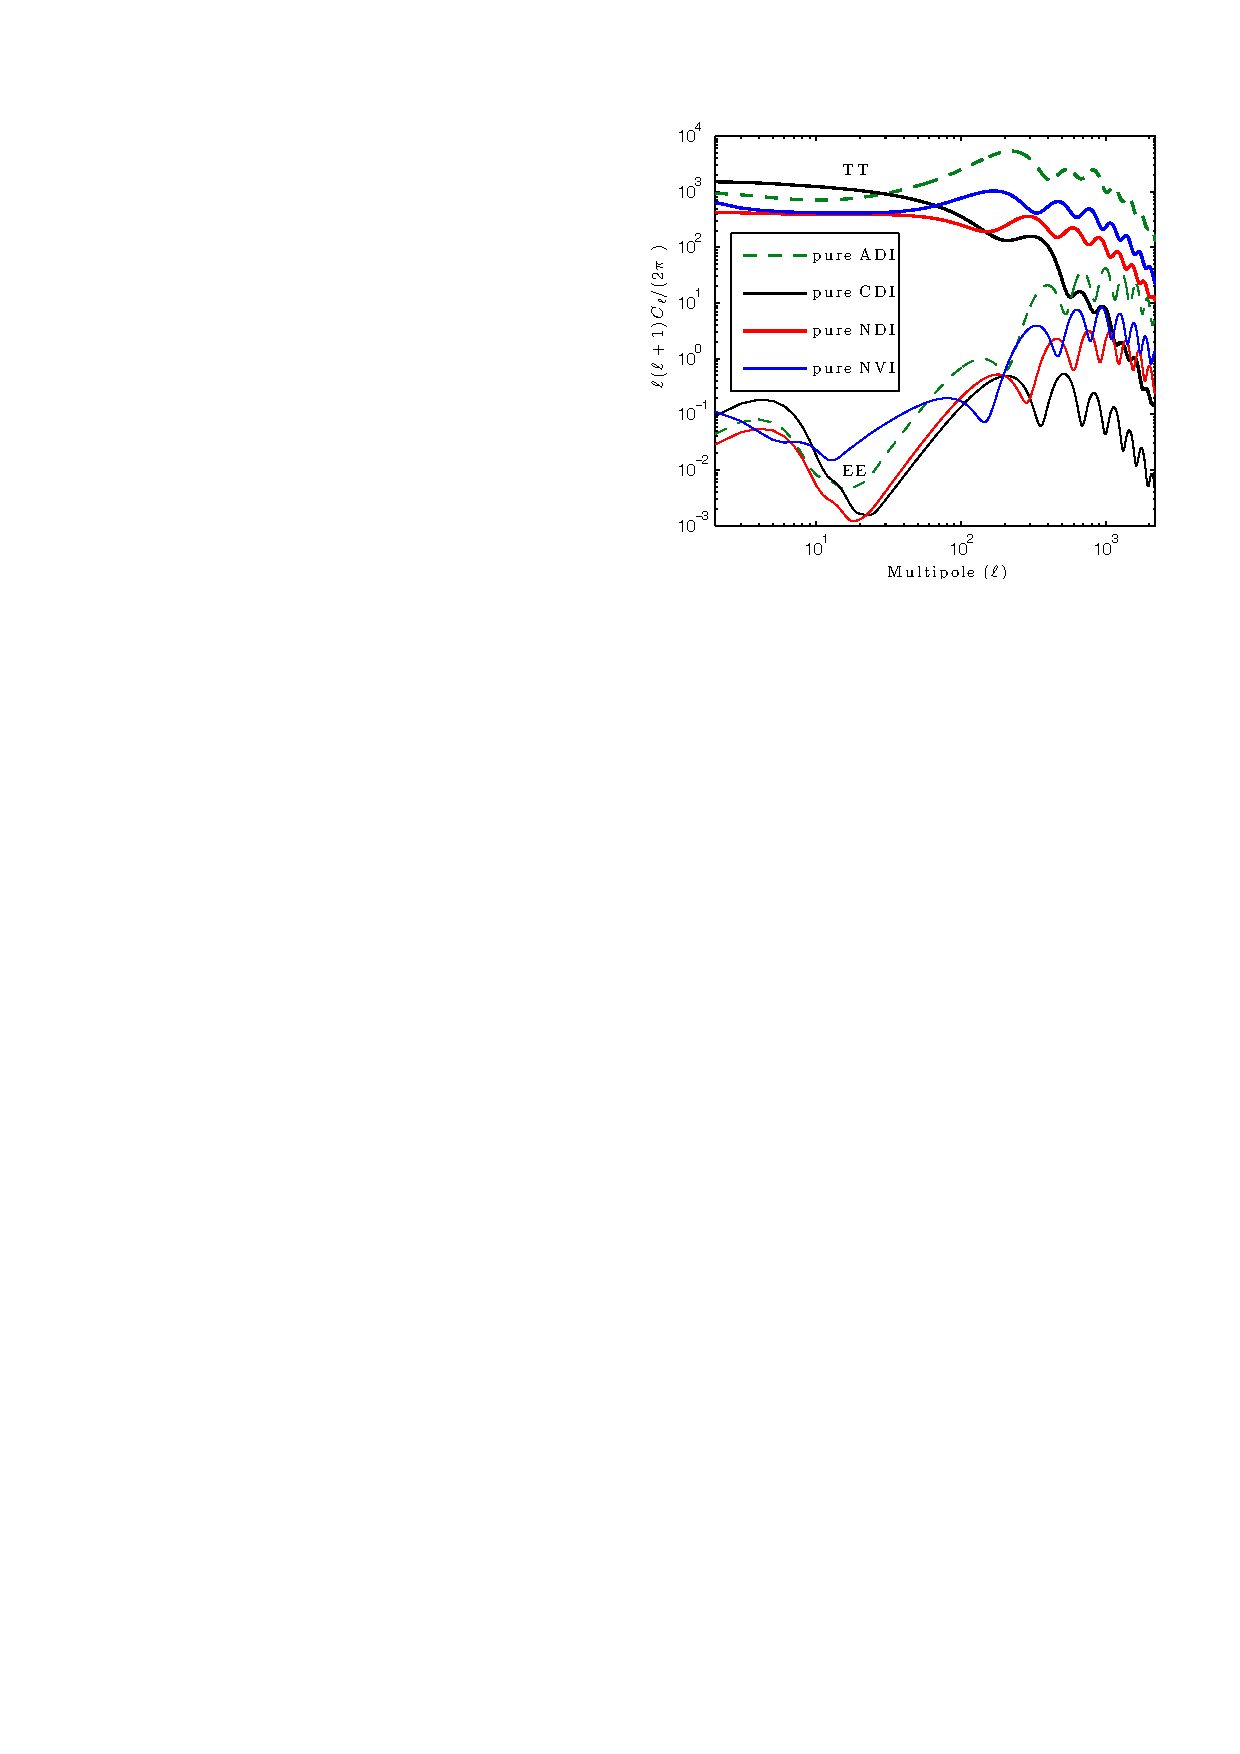
\includegraphics[width=0.5\textwidth, trim={0 10 0 0},clip]{Inflation/iso_schematic.pdf} 
 \caption{CMB isocurvature power spectra $C_{l}^{\rm TT}$ (solid) and $C_{l}^{\rm EE}$ (dashed) for equal primordial $P_{\zeta\zeta}(k)$  isocurvature perturbations. \textbf{Figure appropriated from Planck inflation paper. To be replaced by our own figure.}
\label{fig:iso_schematic}}
\end{figure*} 

Data from WMAP \cite{dunkley09}, \textit{Planck} \cite{Ade:2015lrj}, and other experiments \cite{Enqvist:2000hp,MacTavish:2005yk} indicate that perturbations are predominantly adiabatic. The limits can stated in terms of the fractional primordial power in each isocurvature mode:\begin{equation}
\beta\equiv \frac{P_{S_{i\gamma}}(k)}{P_{S_{i\gamma}}(k)+P_{\zeta\zeta}(k)}.
\end{equation}
The current CMB limits (allowing one isocurvature mode at a time) are shown in Table \ref{table:fisher_model_independent}, along with a forecast of CMB-S4 sensitivity.\footnote{All forecasts in the isocurvature section are produced using Fisher-matrix techniques.} In Table. \ref{table:fisher_model_independent}, ``correlated'' refers to totally correlated or anti-correlated (with $\zeta$) isocurvature perturbations. All results are quoted at a fiducial $k=0.05~{\rm Mpc}^{-1}$. Limits to BDI perturbations are not separately listed, as at linear order they are indistinguishable from CDI perturbations \cite{Gordon:2002gv,Lewis:2002nc,Lewis:2007kz,Gordon:2009wx}. CMB-S4 could improve on these limits by a factor of $2-5$, as shown in Table. \ref{table:fisher_model_independent}.

\begin{table}
\begin{center}
\begin{tabular}
{lcccc}\hline \hline {\rm Mode} &  $ \beta $ (\emph{Planck}, uncorrelated )&$ \beta$(CMB-S4, uncorrelated)&  $ \beta $ (\emph{Planck}, correlated )&$ \beta$(CMB-S4, correlated)\\ 
\hline \\
CDI & $\leq 0.04$&$0.008$&$\leq0.001$&$4\times 10^{-4}$\\
NDI &  $\leq 0.01$ &$XX$&$XX$&$XX$\\
NVI &  $\leq 0.04$&$XX$&$XX$&$XX$\\
\\ \hline \hline 
\end{tabular}
\caption{Constraints (from \emph{Planck} \cite{Ade:2015lrj}) TT+BAO+LowP data vs. CMB-S4 sensitivity to fractional primordial isocurvature power $\beta$ ($95\%$ C.L.) in various modes for uncorrelated/correlated isocurvature modes.\textbf{Numbers to be finalised based on results of Fisher forecast efforts.}
\label{table:fisher_model_independent}}
\end{center}
\end{table} 

\subsection{The Curvaton Scenario}
One alternative to single-field models is the curvaton scenario, in which a sub-dominant second field $\sigma$ acquires vacuum fluctuations during inflation, becomes more important later, sources $\zeta$, and then decays \cite{Mollerach:1989hu,Mukhanov:1990me,Moroi:2001ct,Lyth:2001nq,Lyth:2002my}. Curvaton candidates include sneutrinos, string moduli, and others \cite{Postma:2002et,Kasuya:2003va,Ikegami:2004ve,Mazumdar:2004qv,Allahverdi:2006dr,Papantonopoulos:2006xi,Mazumdar:2010sa,Mazumdar:2011xe}. Depending on whether a species $i$ (or its quantum numbers ) is produced by, before, or after curvaton decay, perturbations in $i$ are offset from $\zeta$, leading to isocurvature perturbations: \cite{Lyth:2001nq,Lyth:2002my,Gordon:2002gv}

\begin{eqnarray}
S_{i \gamma}=\left\{\begin{array}{ll}-3\zeta-3(\zeta_{\gamma}-\zeta),&\mbox{if $i$ is produced before $\sigma$ decay,}\\3\left(\frac{1}{r_{D}}-1\right)\zeta-3(\zeta_{\gamma}-\zeta),&\mbox{if $i$ is produced by $\sigma$ decay},\\ -3(\zeta_\gamma-\zeta),&\mbox{if $i$ is produced after $\sigma$ decay},\end{array}\right.\label{eq:strew}.
\end{eqnarray} Here $\zeta_{i}$ is the density perturbation in $i$ on surfaces of constant curvature. The parameter $r_{\rm D}$ is the fractional energy density in the curvaton when it decays. 

The mixture of isocurvature modes is determined by whether or not baryon number, lepton number, and CDM are produced before, by, or after curvaton decay. Curvaton-type isocurvature is distinct from axion isocurvature, as it is correlated (or anti-correlated) $\zeta$. If lepton number is produced by curvaton decay, the lepton chemical potential $\xi_{\rm lep}$ is important in setting the amplitude of NDI modes \cite{Lyth:2002my,Gordon:2003hw,DiValentino:2011sv}:
\begin{equation}
S_{\nu \gamma}=
-\frac{135}{7}\left(\frac{\xi_{\rm lep}}{\pi}\right)^2\zeta_{\gamma}.\end{equation}
There are $27$ distinct curvaton decay scenarios, as baryon number, lepton number, and CDM could each be produced before, by, or after curvaton decay. Viable models are those in which one of baryon number or CDM is produced by curvaton decay, and those in which \textit{both} baryon number and CDM are produced after curvaton decay. For curvaton-decay scenarios, we use the notation ($b_{x}$, $c_{y}$, $L_{z}$), where $x\in ({\rm before, by, after})$. Here $b$ denotes baryon number, $c$ denotes CDM, and $L$ denotes lepton number. For example, $(b_{\rm before}, c_{\rm by}, L_{\rm by})$ is a model in which baryon number is produced before curvaton decay, CDM by curvaton decay, and lepton number by curvaton decay.

Current isocurvature limits favor values of $r_{\rm D}\simeq 1$, except for models in which baryon number is produced by curvaton decay and CDM before (or vice versa), which favor central values of $r_{\rm D} \simeq 0.16$ ($r_{\rm D} \simeq 0.84$). 

The current limits \cite{Smith/Grin:2015} to $r_{\rm D}$ are shown in Table \ref{limits_rd}, along with a forecast of CMB-S4's sensitivity to $r_{\rm D}$ via isocurvature. The dramatic improvement in the $(b_{\rm by},c_{\rm before},L_{\rm by})$ and $(b_{\rm before},c_{\rm by},L_{\rm by})$ scenarios because of the accompanying NDI perturbations. One unusual case is the $(b_{\rm after},c_{\rm after}, L_{y_{\rm L}})$ scenario. Here isocurvature just constrains the degenerate combination \cite{Smith/Grin:2015} $\chi_{\rm D} \equiv \left\{1+\xi_{\rm lep}^2/(\pi^2) \left(1/r_D -1\right)\right\}^{-1}$, while the independent constraint to $\xi_{\rm lep}^{2}$ is driven by the $N_{\rm eff}$ limit from the CMB.

\begin{table}
\begin{center}
\begin{tabular}
{lcc}\hline \hline {\rm scenario} &  $ \Delta r_D/r_{D}^{\rm adi}$ (\emph{Planck})&$ \Delta r_D/r_{D}^{\rm adi}$(CMB-S4)\\ 
\hline \\
$(b_{\rm by},c_{\rm before},L_{y_{L}})$ & $0.03$&$0.005$\\
$(b_{\rm before},c_{\rm by},L_{y_{L}})$ &  $0.01$ &$0.004$\\
$(b_{\rm by},c_{\rm after},L_{y_{L}})$ &  $0.04$&$0.01$\\
$(b_{\rm after},c_{\rm by},L_{y_{L}})$ & $0.008$&$0.002$\\
$(b_{\rm by},c_{\rm by},L_{y_{L}})$ &  $0.007$&$0.002$\\\hline \hline \\ & $\Delta \chi_{\rm D}/\chi_{\rm }^{\rm adi}$ (\emph{Planck})&$\Delta \chi_{\rm D}/\chi_{\rm }^{\rm adi}$ (CMB-S4) \\\hline \\
$(b_{\rm after},c_{\rm after},L_{y_{L}})$ & $0.003$&$0.0004$\\
\\ 
\end{tabular}
\caption{Isocurvature constraints on $r_D$ ($95\%$ C.L.) using \textit{Planck} TT+BAO+LowP data \cite{Smith/Grin:2015} in viable curvaton decay-scenarios, and Fisher forecasts for CMB-S4 sensitivity. \textbf{Numbers to be finalised based on the final Fisher forecasts as part of larger forecast effort}.
\label{limits_rd}}
\end{center}
\end{table}

\begin{table}
\begin{center}
\begin{tabular}
{lcc}\hline \hline {\rm scenario} &  $\Delta \xi^{2}_{\rm lep}$ (\emph{Planck})&$\Delta \xi^{2}_{\rm lep}$ (CMB-S4) \\ 
\hline \\
$(b_{\rm by},c_{\rm before},L_{\rm by})$ &$0.02$ &$0.002$\\
$(b_{\rm before},c_{\rm by},L_{\rm by})$ &$0.4$  & $0.04$\\
$(b_{\rm by},c_{\rm after},L_{\rm by})$ &$0.3$  &$0.04$\\
$(b_{\rm after},c_{\rm by},L_{\rm by})$ & $0.3$&$0.04$\\
$(b_{\rm by},c_{\rm by},L_{\rm by})$ & $0.3$ & $0.04$\\
$(b_{\rm after},c_{\rm after},L_{\rm by})$ & $0.3$ & $0.04$\\
\\ \hline \hline 
\end{tabular}
\caption{Isocurvature constraints on $\xi_{\rm lep}^{2}$ ($95\%$ C.L.) using \textit{Planck} TT+BAO+LowP data \cite{Smith/Grin:2015} in viable curvaton decay-scenarios where lepton number is generated by curvaton decay, and Fisher forecasts for CMB-S4 sensitivity.\textbf{Numbers to be finalised in forecasting effort.}
\label{limits_xilep}}
\end{center}
\end{table}

Depending on the scenario, forecasting shows that the S4 sensitivity to curvaton-sourced isocurvature should improve by a factor of $2-4$ on current limits. In models with nearly-canceling CDM and baryon isocurvature perturbations, S4 limits to neutrino isocurvature drive an improvement in the sensitivity to the lepton asymmetry from $\Delta \xi_{\rm lep}^{2}\simeq 0.015$ to $\Delta \xi_{\rm lep}^{2}\simeq 0.003$. This dramatic improvement would make CMB limits comparably sensitive to BBN probes $\xi_{\rm lep}^{2}$ (for this decay scenario).

If baryon number/CDM are produced by/before curvaton decay (or vice versa), a relative large compensated isocurvature perturbation (CIP) is produced between the baryons and CDM, that is
\begin{equation}
S_{bc}=\frac{\delta n_{\rm b}}{n_{\rm b}}-\frac{\delta n_{\rm c}}{n_{\rm c}}\neq 0.
\end{equation} Curvaton-generated CIPs are proportional to $\zeta$, $S_{\rm bc}=A\zeta$, where $A\simeq 17$ [$A\simeq -3$] in the $(b_{\rm by}, c_{\rm before}, L_{\rm z})$ [$(b_{\rm before}, c_{\rm by}, L_{\rm z})$] scenario. For CIPs, the initial relative densities of baryons and CDM vary, but with no additional overall matter or radiation density fluctuation.
CIPs are relatively unconstrained at the level of the CMB power-spectrum (see Ref. \cite{Munoz:2015fdv} for an exception), but would induce non-Gaussianities in the CMB \cite{Grin:2011nk,Grin:2011tf,Grin:2013uya,He:2015msa}. As with weak gravitational lensing \cite{Hu:2001kj}, the CIP field $\Delta(\hat{n})$ can be reconstructed using CMB data. We find that at S4 sensitivity \cite{He:2015msa}, the threshold for a $95\%$ C.L. detection is $A\simeq 10$, and so a CIP test of the $(b_{\rm by}, c_{\rm before}, L_{\rm z})$ scenario is within reach of CMB-S4. This is a vast improvement over \emph{Planck} sensitivity, which at $95\%$ C.L. is $A\simeq 43$. Uncorrelated CIPs are less  motivated theoretically. Updating the analysis of Ref. \cite{He:2015msa} with current parameters \cite{Ade:2015lrj} and CMB-S4 specifications, we find that the sensitivity of CMB-S4 to a scale-invariant (SI) angular power spectrum of uncorrelated CIPs is $\Delta_{\rm cl}=0.003$ at the $95\%$ C.L. detection limit. Here $\Delta_{\rm cl}$ is the r.m.s. CIP amplitude on cluster scales. This is a vast improvement over the upper limit of $\Delta_{\rm cl}\leq 0.077$ from WMAP \cite{Grin:2013uya}, or the forecasted Planck \cite{Ade:2015lrj} (including polarization) sensitivity of $\Delta_{\rm cl}\leq 0.015$ \cite{He:2015msa}.


%We now focus on two isocurvature scenarios, axion dark matter and the curvaton %model, which produce uncorrelated and correlated isocurvature pertrubrations, %respectively.



%% Populate the .bib file with entries from SPIRES Bibtex (preferred)
%% or ADS Bibtex (if no SPIRES entry).
%%  SPIRES will also supply the CITATION line information; please include it.
%%

\section{Summary}
CMB-S4 is an ideal tool to test the inflationary paradigm and competing theories of the early universe. On the one hand, its exquisite sensitivity will allow a detection of degree scale B-modes in the CMB or achieve upper limits on the amount of B-mode polarization that improve current constraints on the tensor-to-scalar ratio by almost two orders of magnitude. In particular, it is sensitive enough to detect the level of B-mode polarization predicted in a wide range of well-motivated inflationary models. In doing so, it would provide invaluable information about physics at energy scales far outside the reach of any terrestrial particle physics experiment. In the absence of a detection it would exclude large classes of inflationary models. On the other hand, with its high angular resolution, it will measure anisotropies in both the temperature and E-mode polarization of the CMB to cosmic variance over the entire range of multipoles that is not contaminated by unresolved foregrounds, and it will extend our window to the early universe by almost one $e$-fold beyond the reach of current experiments. As a consequence, it will provide the best constraints achievable by any ground-based CMB experiment on any observable that benefits from the number of modes measured, such as the primordial power spectrum, and hence the spectral index, its running, features in the power spectrum, as well as higher order correlations.


 
